\label{sec:FD_control}
\section{\onedof\ system}
From now on, the controllers synthesis and simulations are based on the \textit{gray-box} model; here is reported the transfer function from the applied voltage to the first mass speed: \\
\[	
G_{v, \dot \theta_1}(s)=
\frac{-5.618 \cdot 10^{4}}{{s^3 + 21.45 s^{2}}+1699 s+3.149 \cdot 10^{4}}
\]

\begin{figure*}[h]
	\centering
	\begin{subfigure}{0.55\columnwidth}
		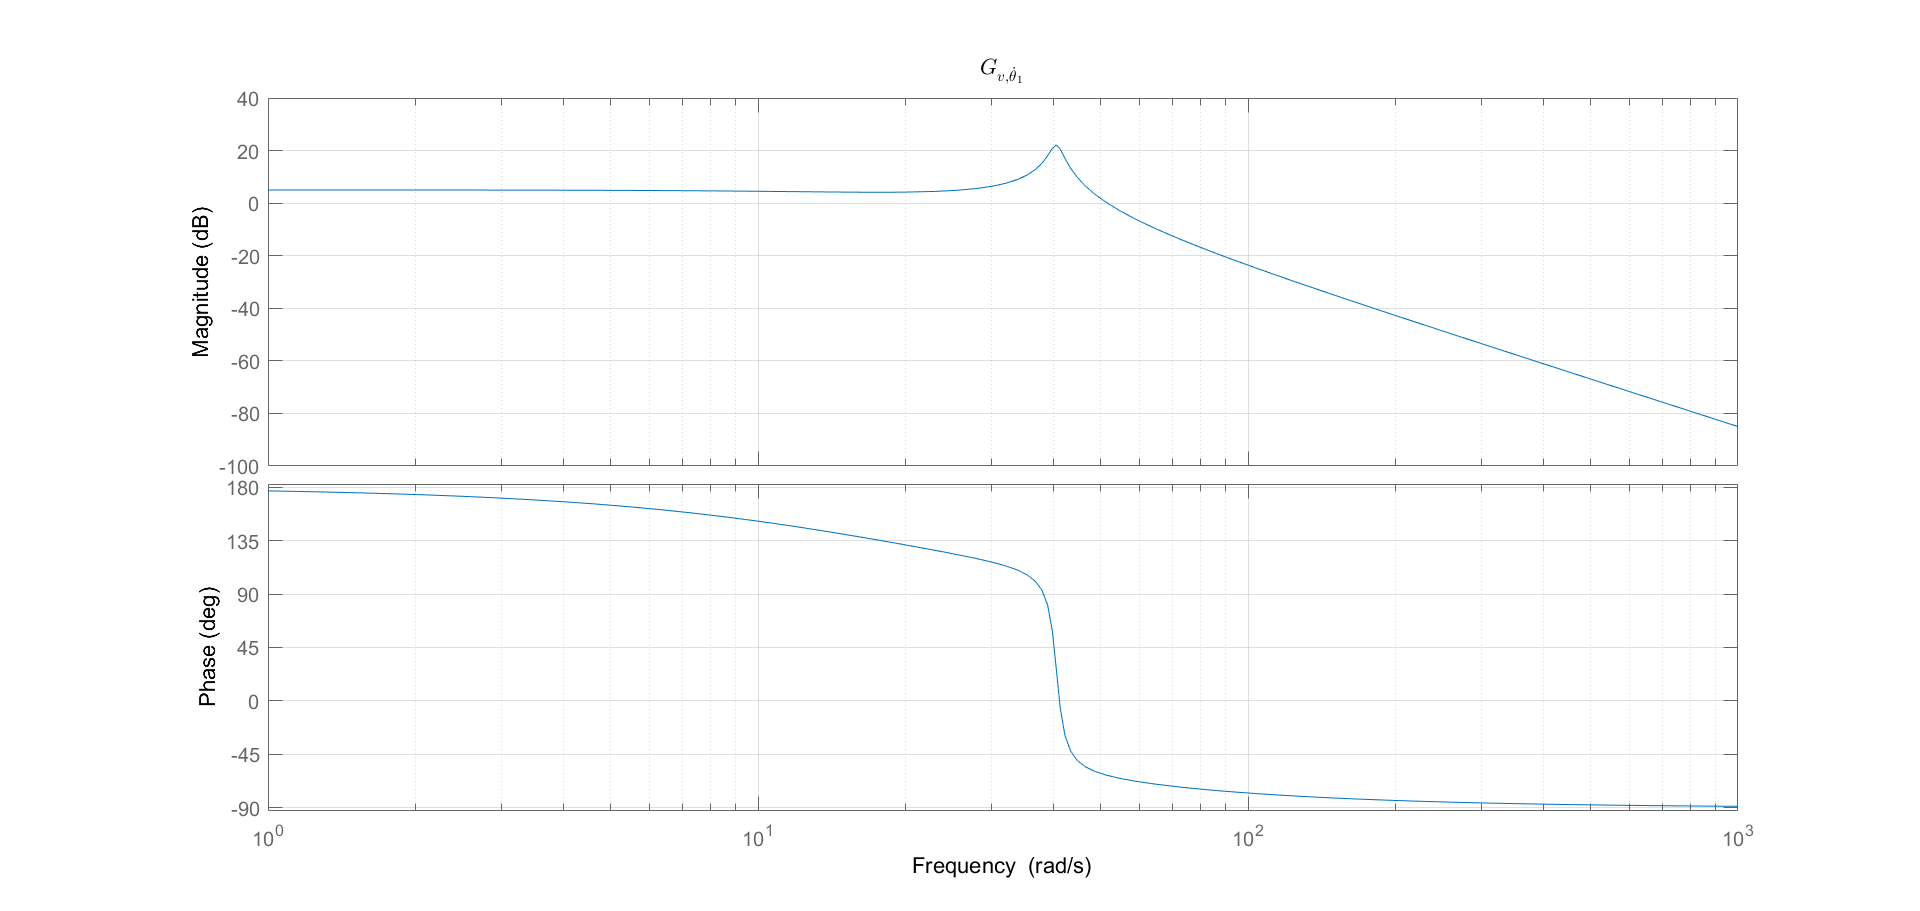
\includegraphics[width=\textwidth]{1Bode_G}
	\end{subfigure}
	\begin{subfigure}{0.4\columnwidth}
		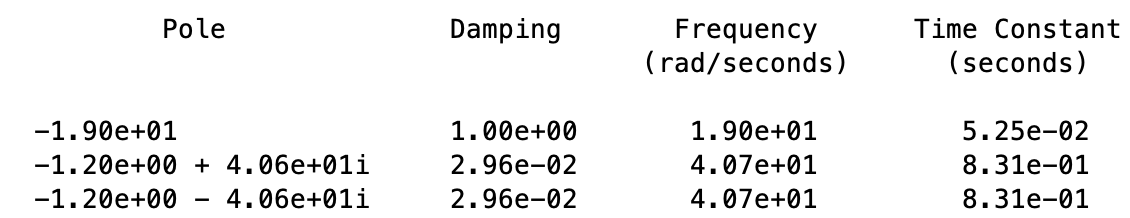
\includegraphics[width=\textwidth]{1Pole_G}
	\end{subfigure}
	\caption{$G_{v, \dot \theta_1}(s)$}
	\label{fig:G(s)1dof}
\end{figure*}

It is possible to notice, in \cref{fig:G(s)1dof}, that there is a couple of complex conjugated poles with low damping coefficient. The proposed solution is to apply a notch filter, thanks to which it is possible to delete these poles and substitute them with a couple of complex conjugated poles at the same frequency, but with a damping coefficient equal to~$0.72$. It has been decided not to alter too much the behavior of the plant to avoid too aggressive control actions, for this reason notch poles haven't been imposed as real poles or as high frequency poles.

\begin{figure*}[h]
	\centering
	\begin{subfigure}{0.47\columnwidth}
		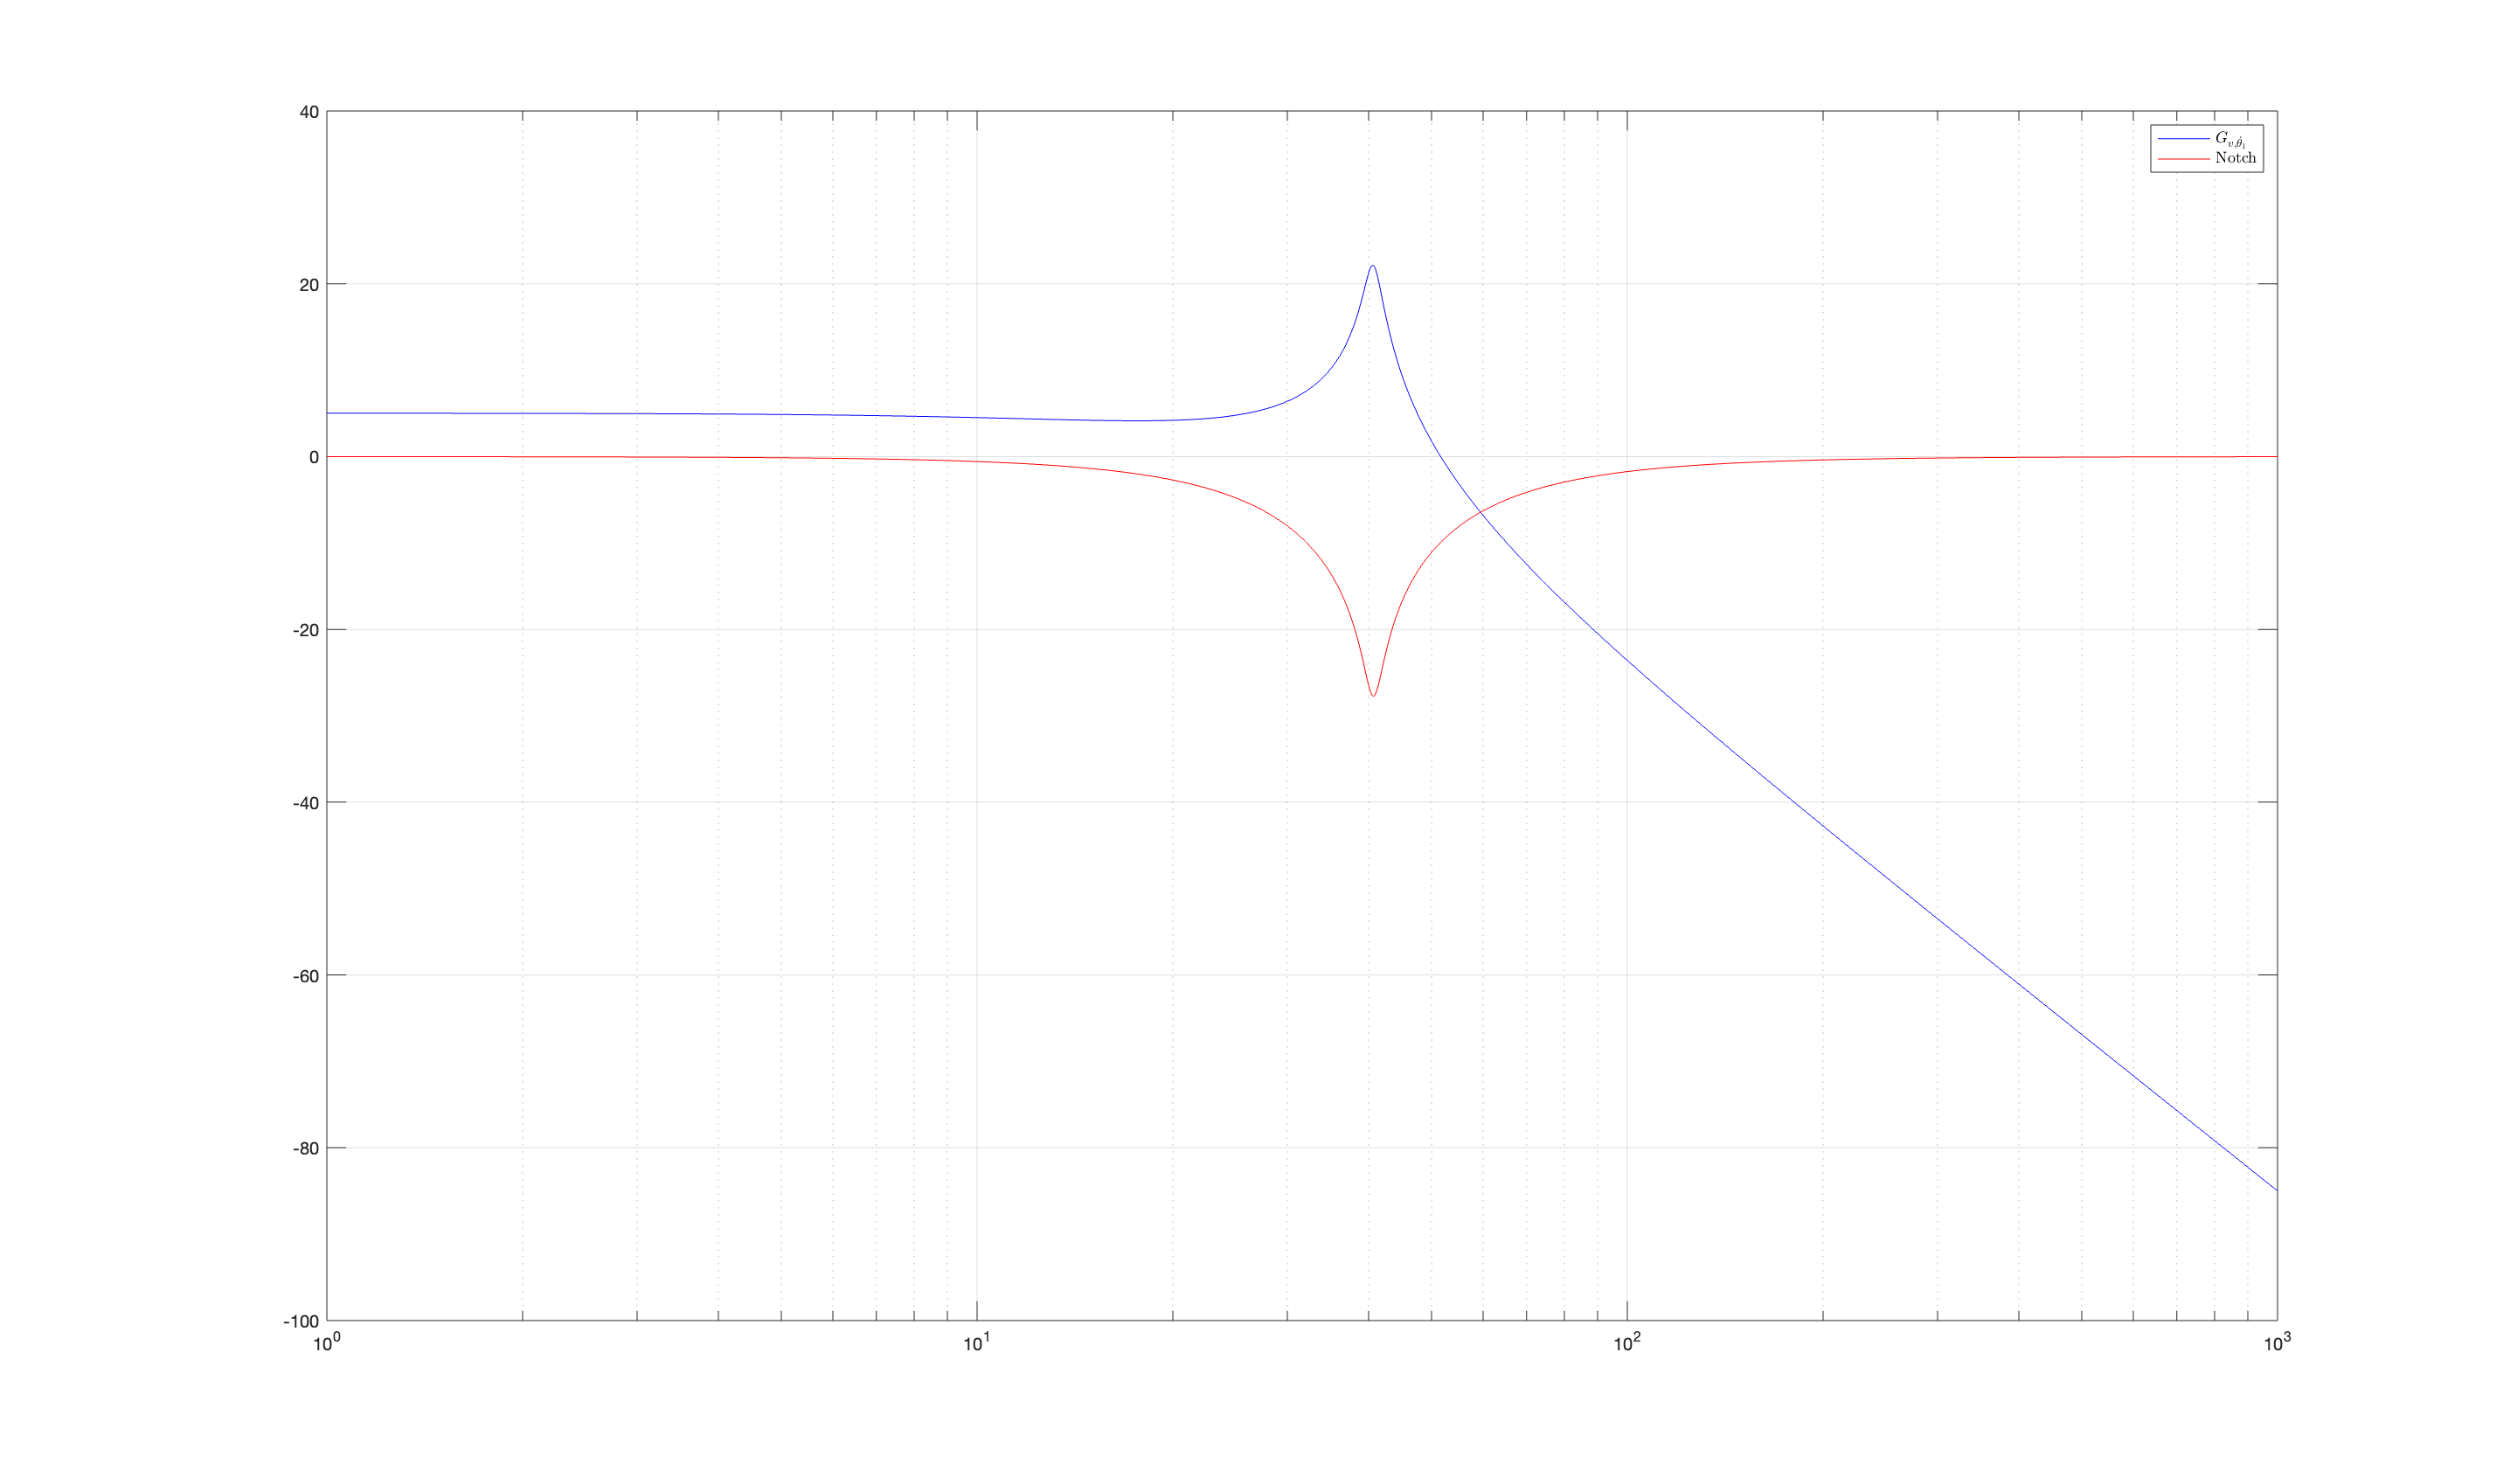
\includegraphics[width=\textwidth]{1Nf_G}
		\subcaption{$N_f(s)$ and $G(s)$}
	\end{subfigure}
	\begin{subfigure}{0.47\columnwidth}
		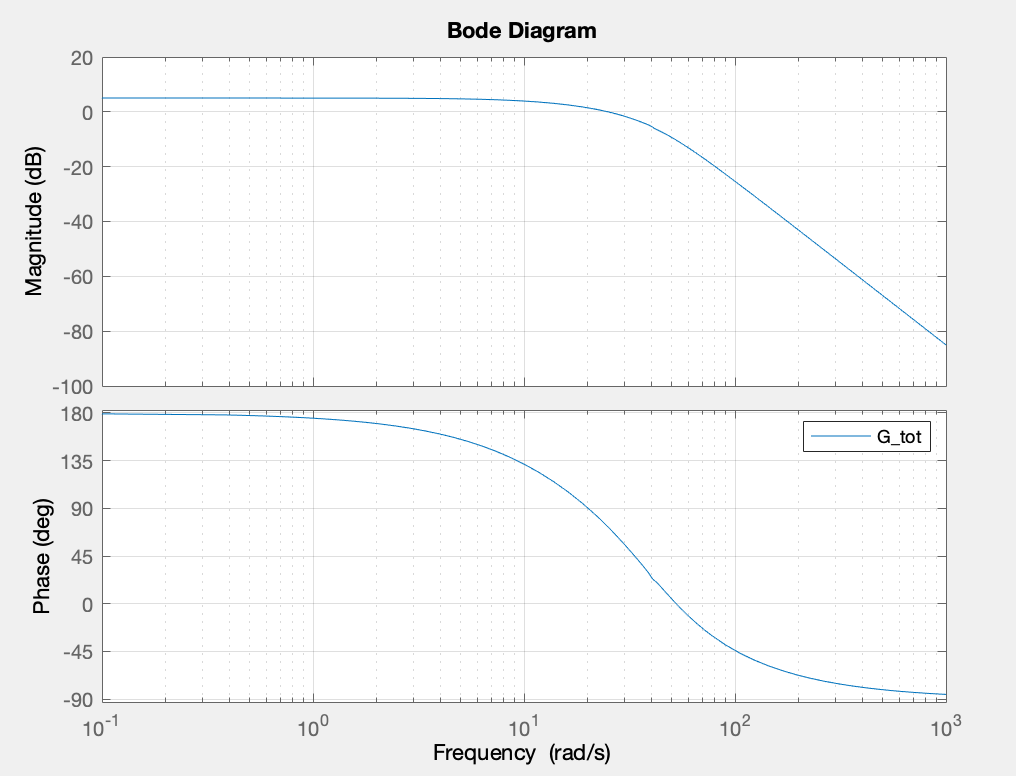
\includegraphics[width=\textwidth]{1_Gtot}
		\subcaption{$G_{tot}(s)$}
	\end{subfigure}
	\caption{Plant $G(s)$ with Notch Filter $N_f(s)$: $G_{tot}(s)$}
	\label{fig:Plant G(s)with Notch Filter1}
\end{figure*}


Applying the notch filter represented in \cref{fig:Plant G(s)with Notch Filter1}(a), the controller now sees the plant $G_{tot}$(s) of \cref{fig:Plant G(s)with Notch Filter1}(b).

\newpage
\subsection{Speed Control Loop}
The selected controller structure is the PI, enriched with an anti-windup structure, that cancels out the real frequency pole at~$19\ rad/s$.
\begin{center}
$ R(s) = -k_v \frac{\frac{s}{19}+1}{s} $,
with \quad
$ k_{v} = \frac{w_{c,v}}{G(0)} $
\end{center}
\begin{figure*}[h]
	\centering
	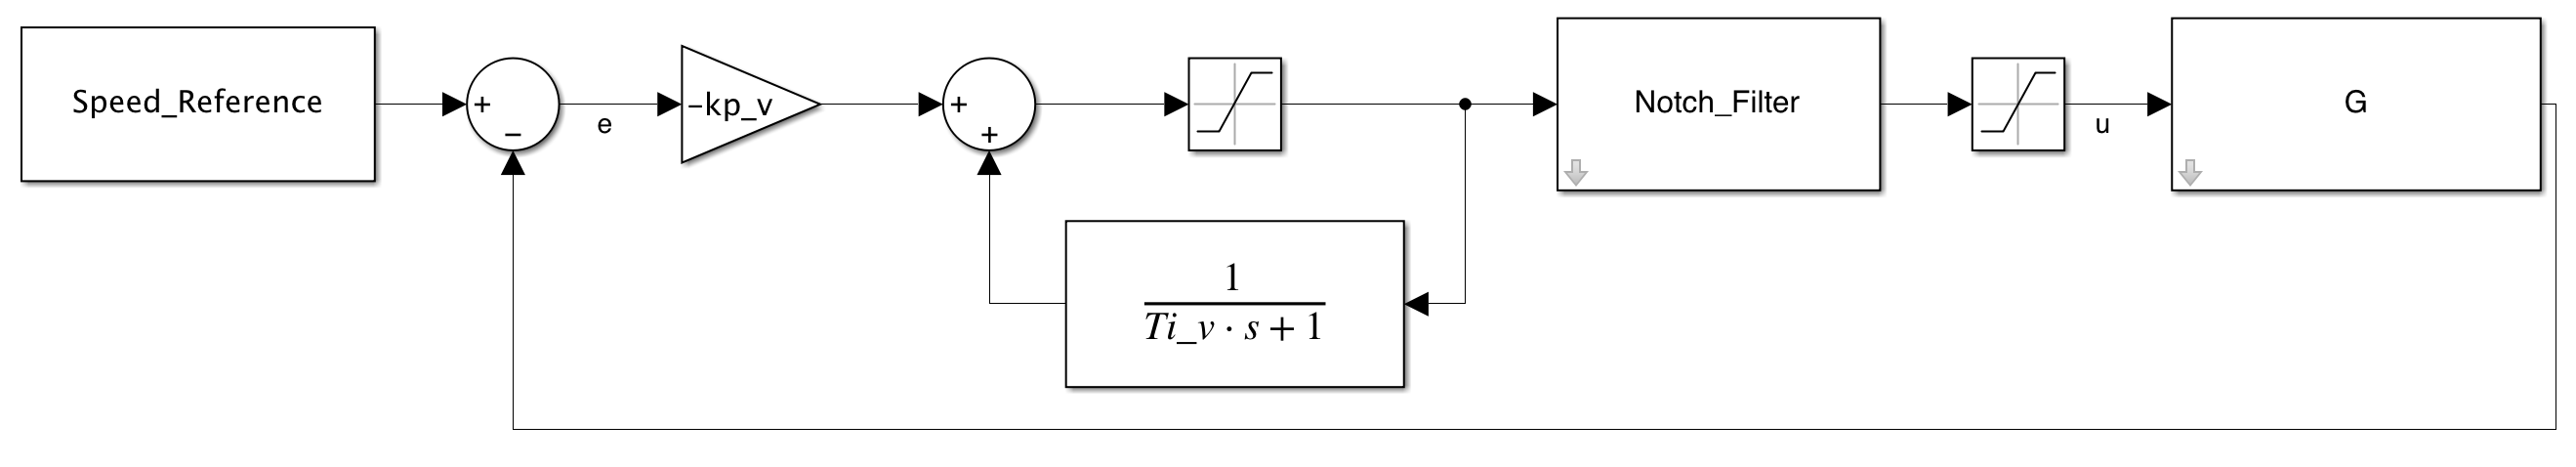
\includegraphics[width=0.8\textwidth]{1dof_PI_scheme}
	\caption{Closed-loop block scheme}
\end{figure*}

\paragraph{Specifications}
The goal of this first controller is to obtain a fast and robust performance. In particular,
\begin{itemize}
	\item settling time: $T_s \leq 0.5\ s$
	\item phase margin: $\phi_m \geq 65\degree$
\end{itemize}

\paragraph{Tuning and simulation}
From now on, $k_v$ will be used as tuning parameter of the PI regulator, while the~$0\ dB$ axis of Bode diagram of speed loop is indicated by~$w_{c,v}$. In order to reach the desired specifications, many Bode analyses and simulations have been done: here are reported cases with~$k_v=3.5$ and~$k_v=4.5$.
\begin{figure*}[h]
	\centering
	\begin{subfigure}{0.45\columnwidth}
		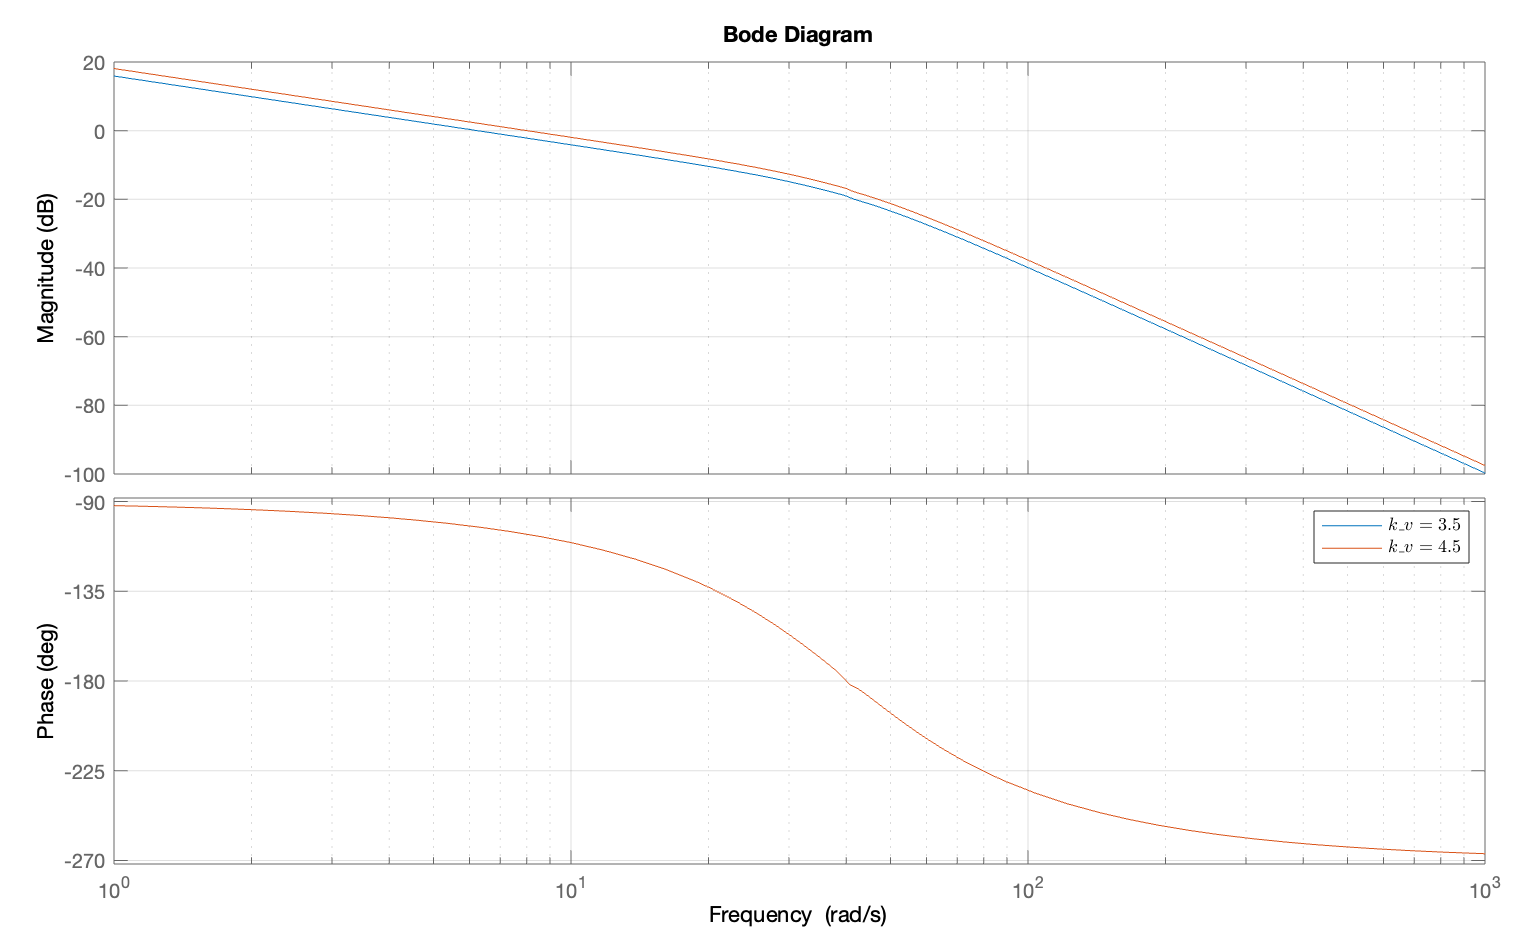
\includegraphics[width=\textwidth]{1dof_bode_trials}
		\subcaption{Open-loop Bode diagrams}
		\label{fig:PI1dof_bode}
	\end{subfigure}
	\begin{subfigure}{0.42\columnwidth}
		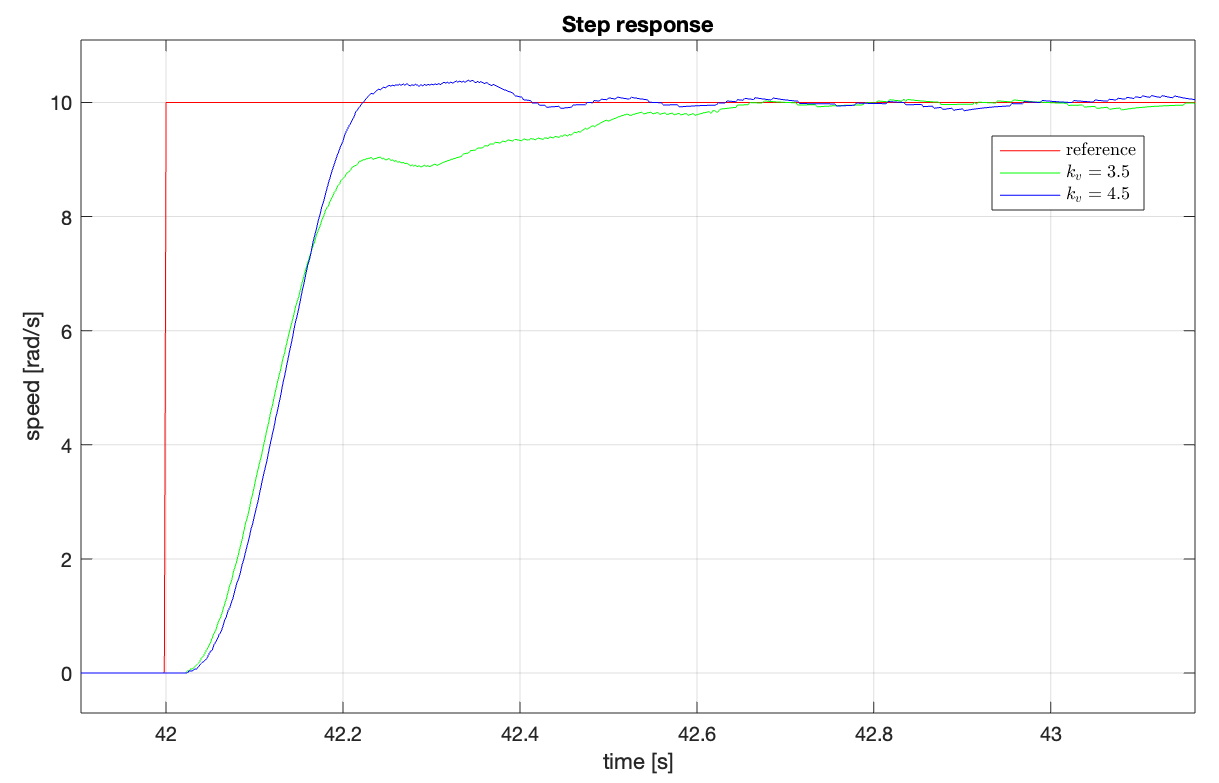
\includegraphics[width=\textwidth]{1dof_step_trials}
		\subcaption{Laboratory data of closed-loop step responses}
		\label{fig:PI1dof_step}
	\end{subfigure}
	\caption{Comparisons between $k_v = 3.5$ and $k_v = 4.5$ cases}
	\vspace{5mm}
	\begin{subfigure}{0.6\columnwidth}
		\centering
		\begin{tabular}{|c|cc|}
			\hline
			Results\footnote{Cutting frequency~$\omega_{c,v}$, gain margin~$G_m$ and phase margin~$\phi_m$ are obtained theoretically by means of MATLAB. Instead, settling time~$T_s$ is measured through data collected at the laboratory.} & $k_v=3.5$ & $k_v=4.5$ \\
			\hline
			$\omega_{c,v}\ [rad/s]$ & $6.24$ & $8.01$ \\
			$G_m\ [dB]$ & $19$ & $16.8$ \\
			$\phi_m\ [deg]$ & $77.3$ & $73.6$ \\
			\hline
			$T_s\ [s]$ & $0.65$ & $0.40$ \\
			\hline
		\end{tabular}
		%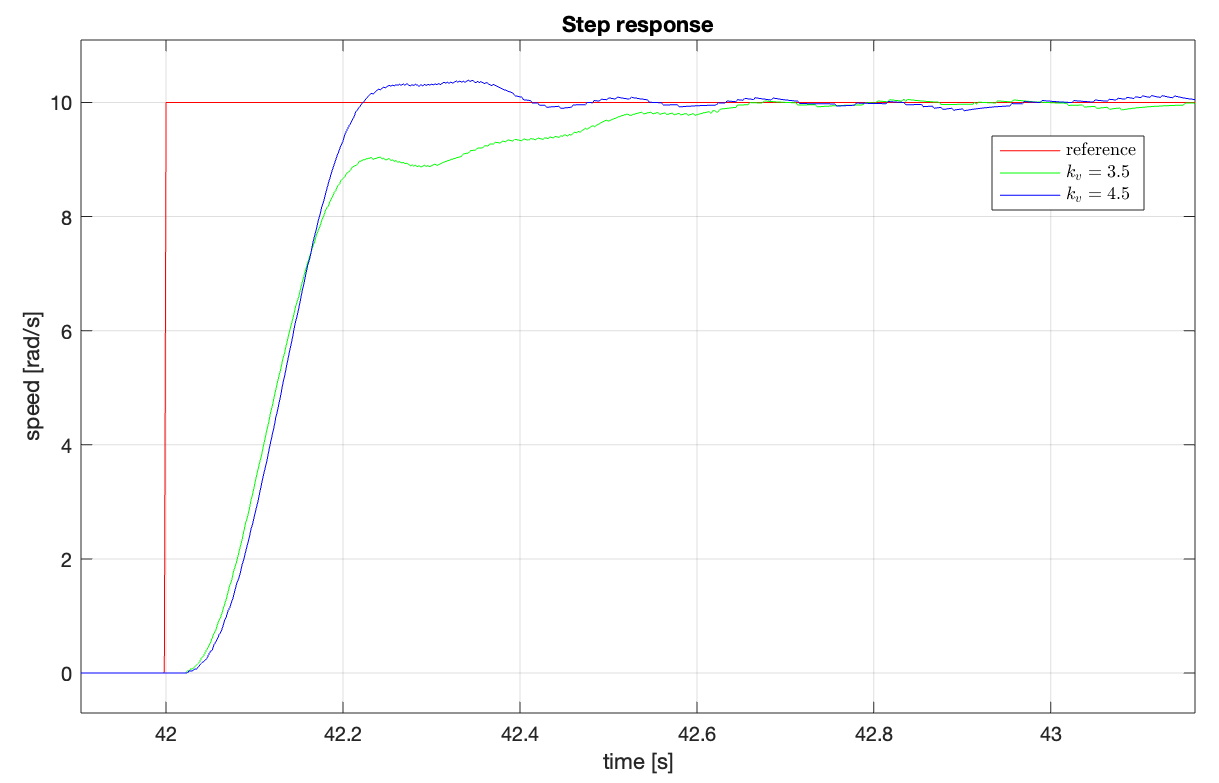
\includegraphics[width=\textwidth]{1dof_step_trials}
		%\caption{Closed-loop step responses}
		%\label{fig:step_PI1dof_step}
	\end{subfigure}
	\caption{Table of theoretical results, $k_v = 3.5$ and $k_v = 4.5$ cases}
	\label{fig:Bode and Step PI 10}
\end{figure*}

\paragraph{Performance analysis}
The only choice that satisfies all the requirements is obtained by imposing~$k_v = 4.5$. To test it, one of the worst case scenarios has been applied, that is the step from~$-17\ rad/s$ to~$17\ rad/s$, and then a smaller step of~$10\ rad/s$. The first one allows to asses the voltage saturation in the worst case, while the second one can be representative of the transient for an ordinary step.
In \cref{fig:PI with 4.5} is shown the comparison between the simulation and the data collected in the laboratory on the real system.
\begin{figure*}[h]
	\centering
	\begin{subfigure}{0.45\columnwidth}
		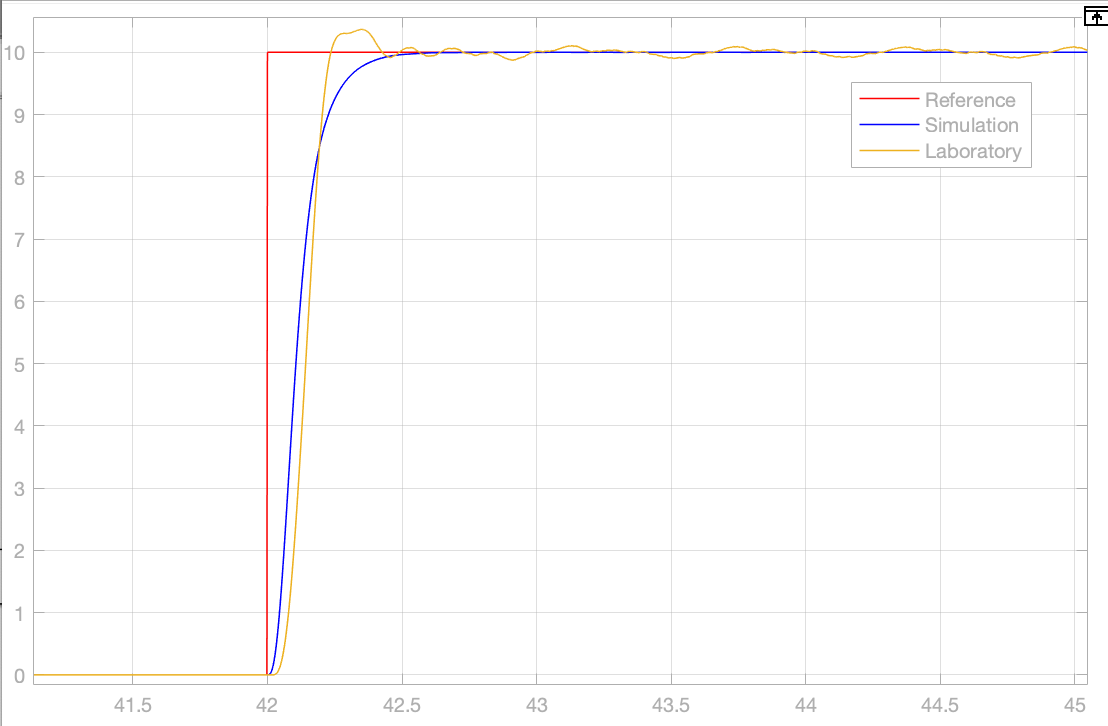
\includegraphics[width=\textwidth]{1_step10}
		\subcaption{Step of $10\ rad/s$}
	\end{subfigure}
	\begin{subfigure}{0.45\columnwidth}
		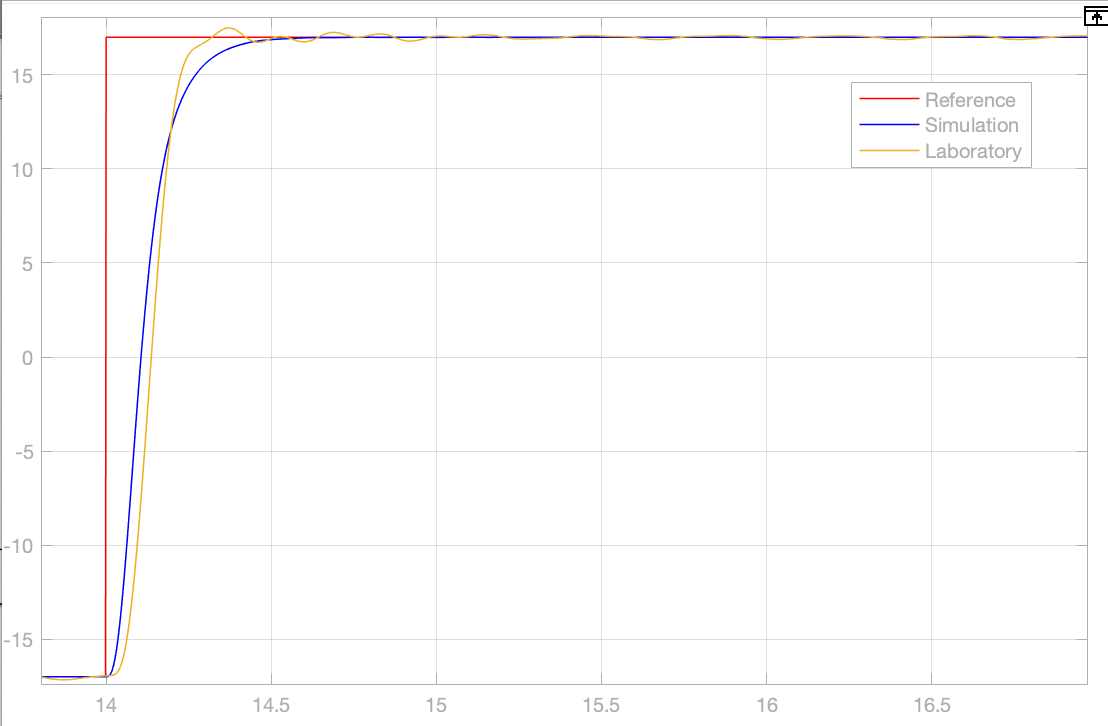
\includegraphics[width=\textwidth]{1_step17}
		\subcaption{Step of $34\ rad/s$}
	\end{subfigure}
	\newline
	\begin{subfigure}{0.45\columnwidth}
		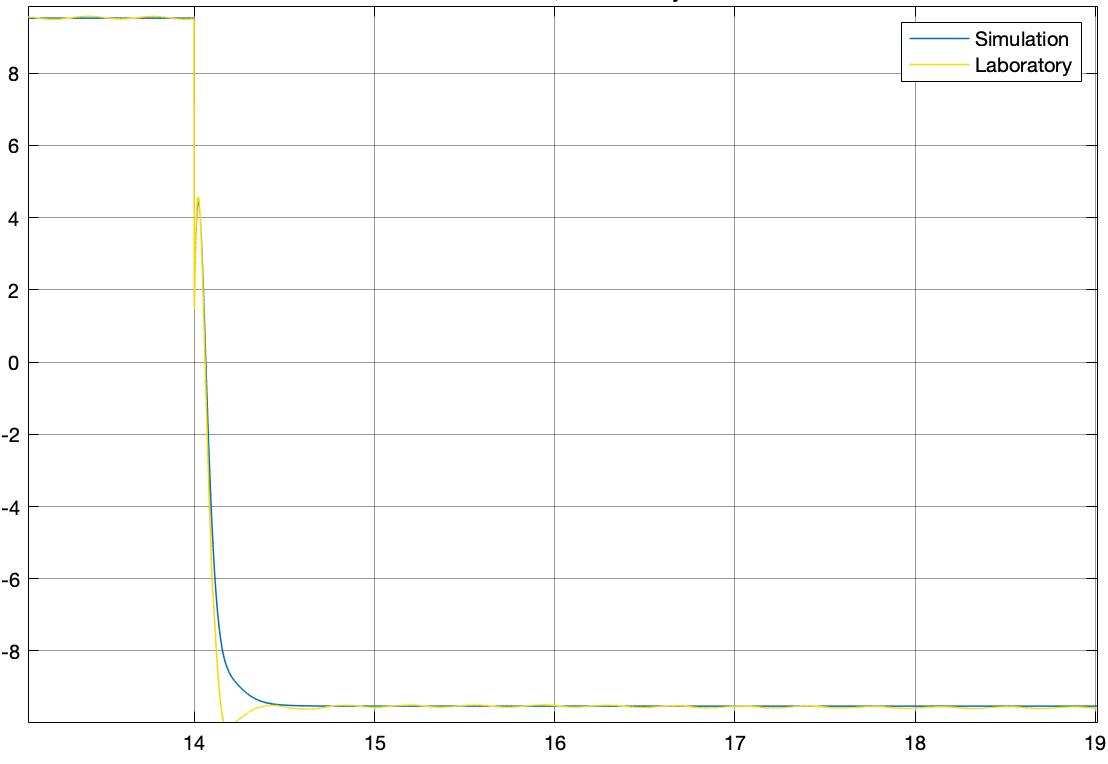
\includegraphics[width=\textwidth]{1_volt17}
		\subcaption{Voltage related to a step of $34\ rad/s$}
	\end{subfigure}
	\caption{Speed control loop with $k_{v}=4.5$}
	\label{fig:PI with 4.5}
\end{figure*}
\subparagraph{Overshoot and phase margin}
In the experimental data, an overshoot appears. This behavior is due to a lower phase margin of the real system, caused by a wrong estimation of the dominant pole, whose frequency might be actually lower than~$19\ rad/s$. \\
This issue allows to compute the phase margin: through the overshoot height percentage ($S_\% = \frac{0.4\ rad/s}{10\ rad/s} = 4\%$), it is possible to compute the system approximation damping~$\xi$ and, so, the phase margin~$\phi_m$ by means of the following formulas.
\begin{equation}
	S_\% = 100\ e^{\frac{-\pi\xi}{\sqrt{1-\xi^2}}} ,
	\qquad
	\phi_m = \frac{180\degree}{\pi} \arctan \Biggl( \frac{2\xi}{\sqrt{-2\xi^2 + \sqrt{1+4\xi^4} }} \Biggr)
\end{equation}
The obtained value is~$\phi_m = 66.2 \degree$, that is considered satisfactory according to our initial specifications.

\subparagraph{Oscillations}
A resonance uncertainty is observable through the small oscillations at the end of the transient, which are not well compensated by the notch filter. \\
Another aspect that has to be considered is the presence of oscillations at steady state. Their frequencies are equal to the speed, then a possible explanation can be a change of the dynamic friction coefficient value along the revolution. As a matter of fact, this undesired behavior can be neglected, since the amplitude of the above-mentioned oscillations is very small. In case is necessary to attenuate them, the bandwidth of the loop should be increased to counteract them on time. By using just a PI as controller this is not possible, because increasing the cutting frequency results in lower phase margin and significant oscillations to the step response, that cannot be accepted. \\
To avoid this behavior to steps in the reference signals, a solution could be placing a low-pass pre-filter on the reference signal. In this way, a step on the speed reference would result in a smoother reference signal and smaller oscillations will arise. This solution is analyzed with more details in the \twodof\ case, where these oscillations at the steady state cannot be neglected.

\paragraph{Bandwidth estimation}
In \cref{fig:sinesweep_PI_1dof} and \cref{fig:Ramp1dof} are shown the responses of the closed-loop system to a sine-sweep, experiment that allows to evaluate its bandwidth, and to a ramp reference with a decreasing slope, that permits to asses the range of reachable speed set-points (especially for what concerns the low speeds). \\
The analysis of both step and closed-loop sine-sweep responses, respectively \cref{fig:PI with 4.5} and \cref{fig:sinesweep_PI_1dof}, it appears that simulations do not follow exactly the data collected in the laboratory. This difference is caused by a non perfect identification of the real system. Indeed, an estimation of the bandwidth from the sine-sweep experiment is performed, two different crossover frequencies are obtained: the simulation places it around~$8.17\ rad/s$ and the real system one appears to be around~$17\ rad/s$. These values have been computed starting from the theory, for which the attenuation at the cutting frequency is~$-3\ dB$. \\
It can be noticed that a small resonance occurs around the cross-over frequency of the real system: a phase margin smaller that~$70 \degree$ can lead to this behavior. \\
Moreover, it cannot be neglected the fact that this is a speed controller. Speed measurement is obtained through the derivation of the position of the encoder. Thus, these bandwidth values are not fully reliable because of uncertainty in measurement.

\begin{figure*}[h]
	\centering
	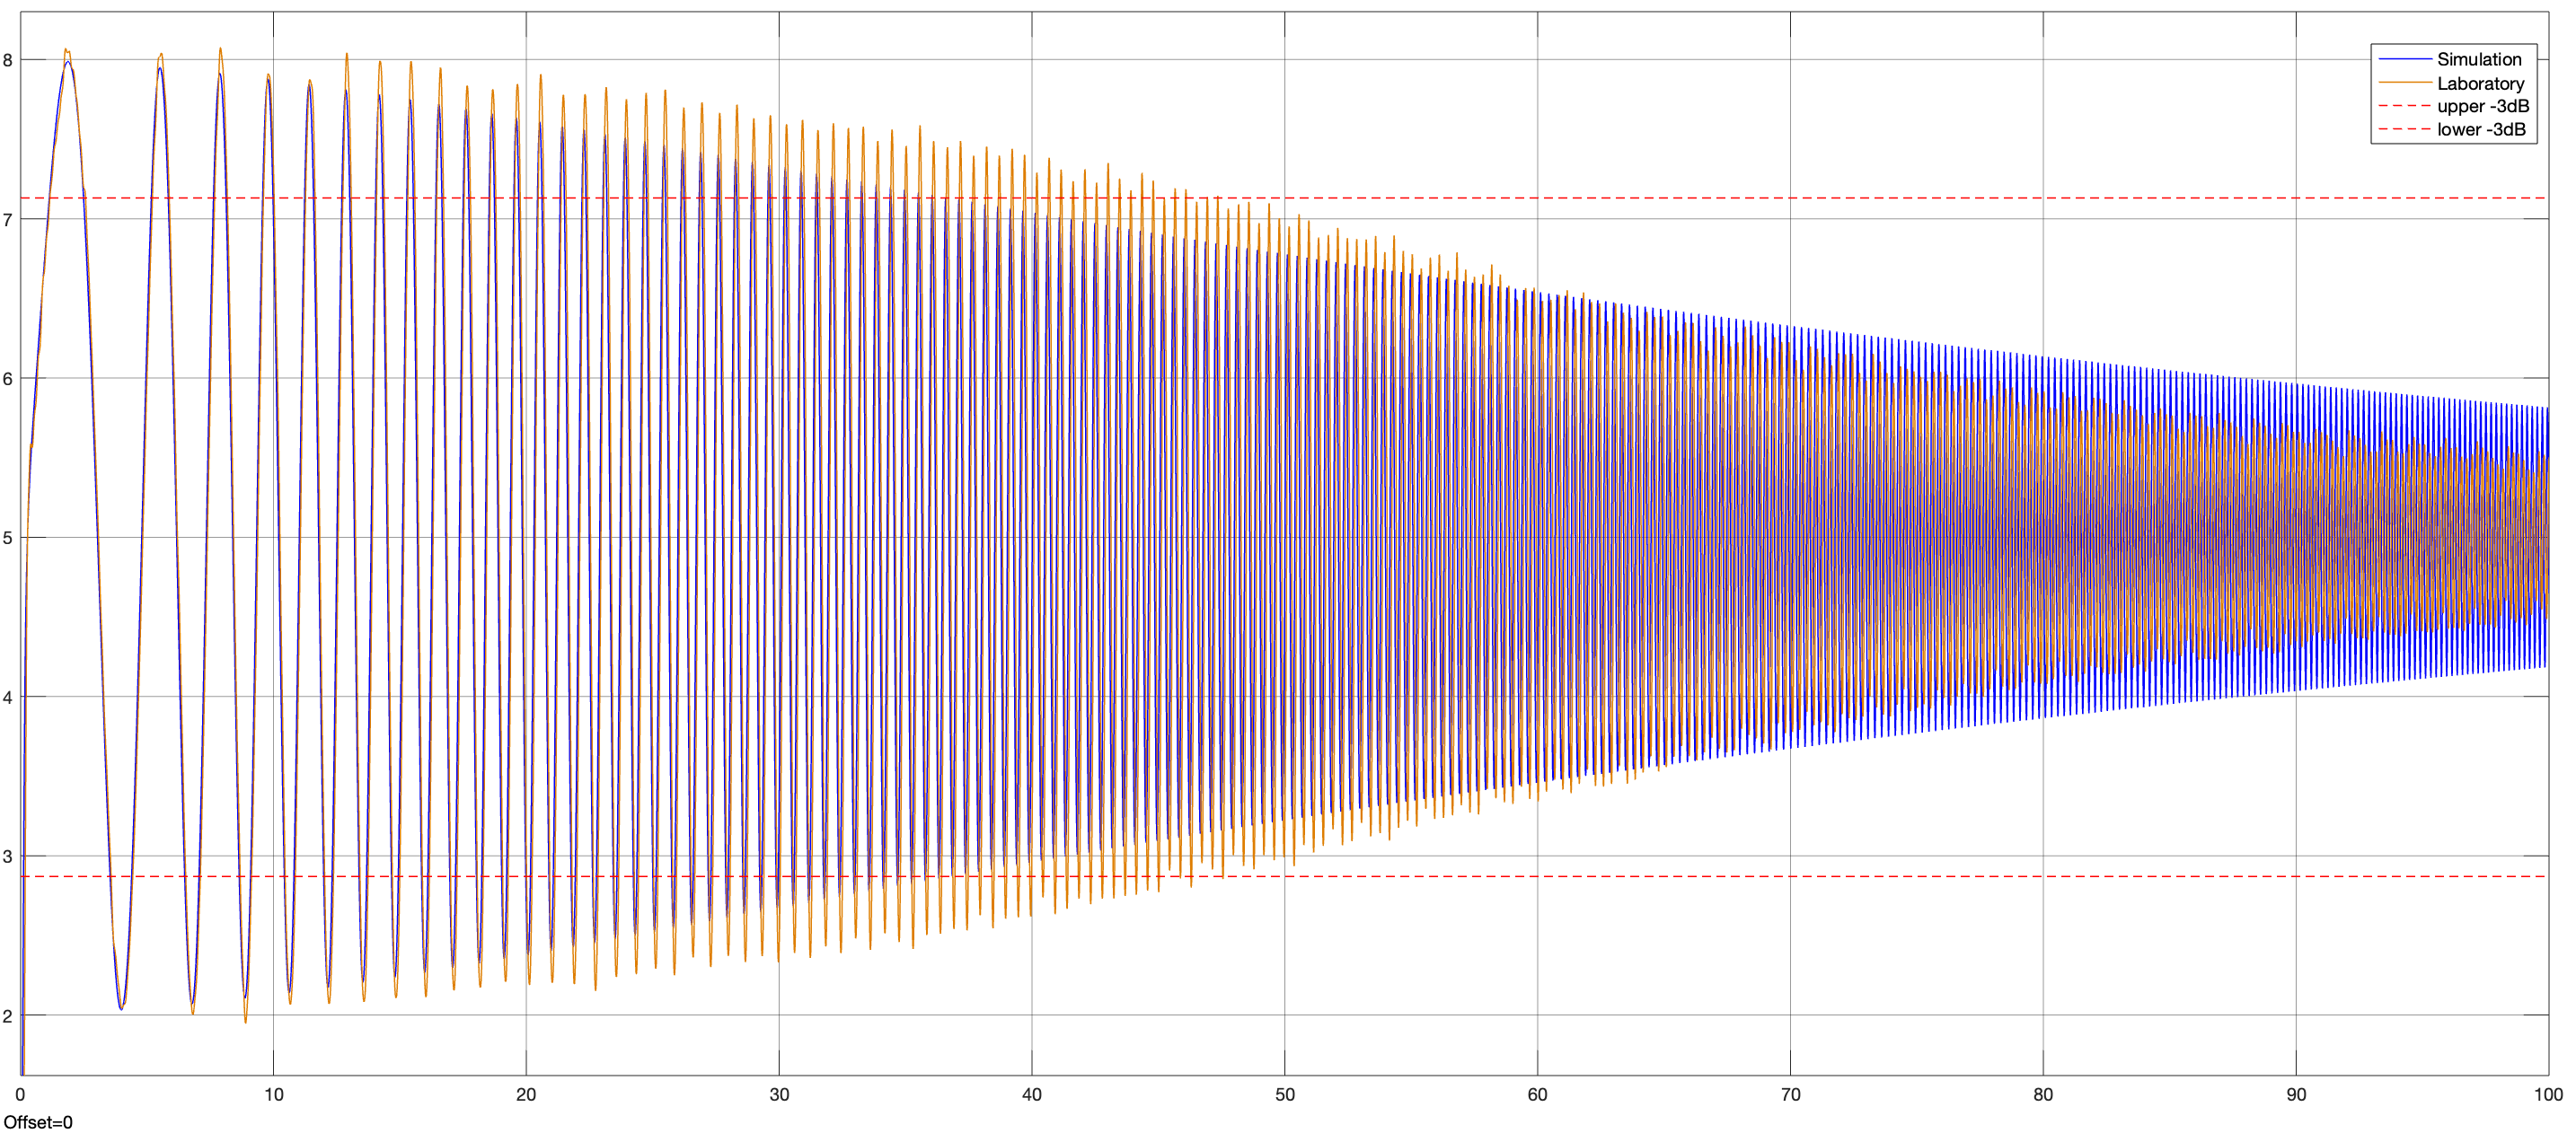
\includegraphics[width=0.9\columnwidth]{Sine1dof}
	\caption{Sineweep experiment from $0.1\ Hz$ to $10\ Hz$ in $100\ s$}
	\label{fig:sinesweep_PI_1dof}
\end{figure*}

\begin{figure*}[h]
	\centering
	\begin{subfigure}{0.4\columnwidth}
		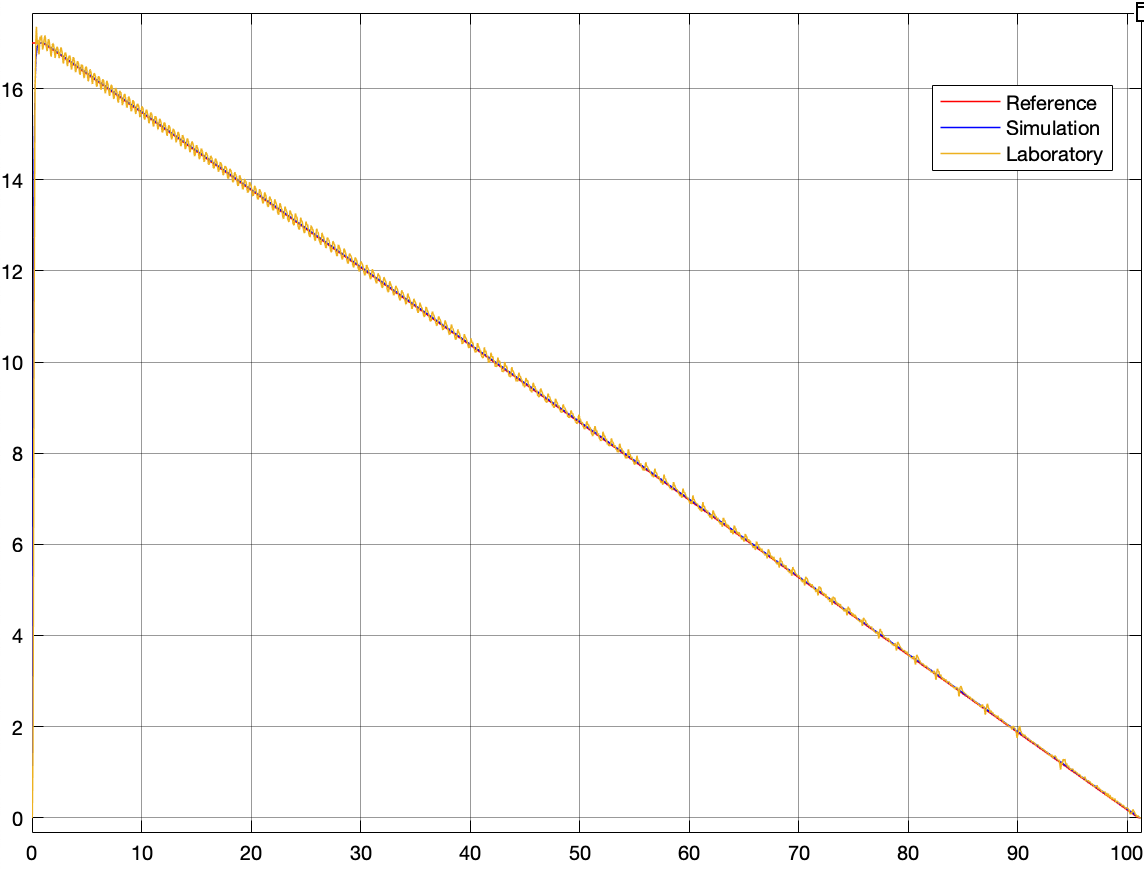
\includegraphics[width=\textwidth]{Ramp1dofa}
		\subcaption{Entire experiment}
	\end{subfigure}
	\begin{subfigure}{0.4\columnwidth}
		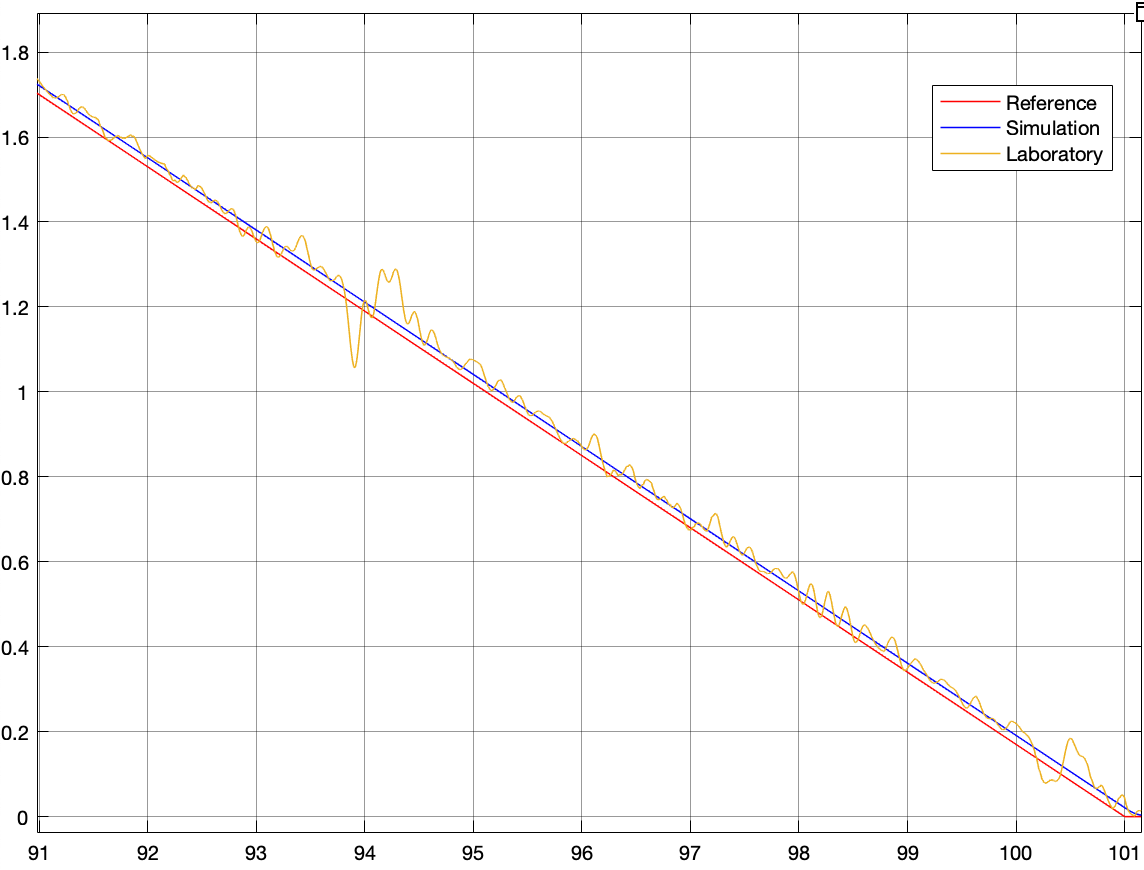
\includegraphics[width=\textwidth]{Ramp1dofb}
		\subcaption{Detail at low speed}
	\end{subfigure}
	\caption{Ramp experiment from $17\ rad/s$ to $0\ rad/s$ in $100\ s$}
	\label{fig:Ramp1dof}
\end{figure*}

Thanks to the ramp experiment, it has been verified that this regulator can control the system even at very low speed. This result is very satisfying, because of the wide controllability range, which goes from~$-17.5\ rad/s$ to~$-0.3\ rad/s$ and from~$0.3\ rad/s$ to~$17.5\ rad/s$.

\newpage
\subsection{Position Control Loop}
To control the position, different techniques have been considered: direct P and PI controllers on the mass position error have been taken into account. Since the speed control loop has highlighted some uncertainties on the model, a cascade control is useful for disturbances rejection and to face uncertainties.
\begin{figure*}[h]
	\centering
	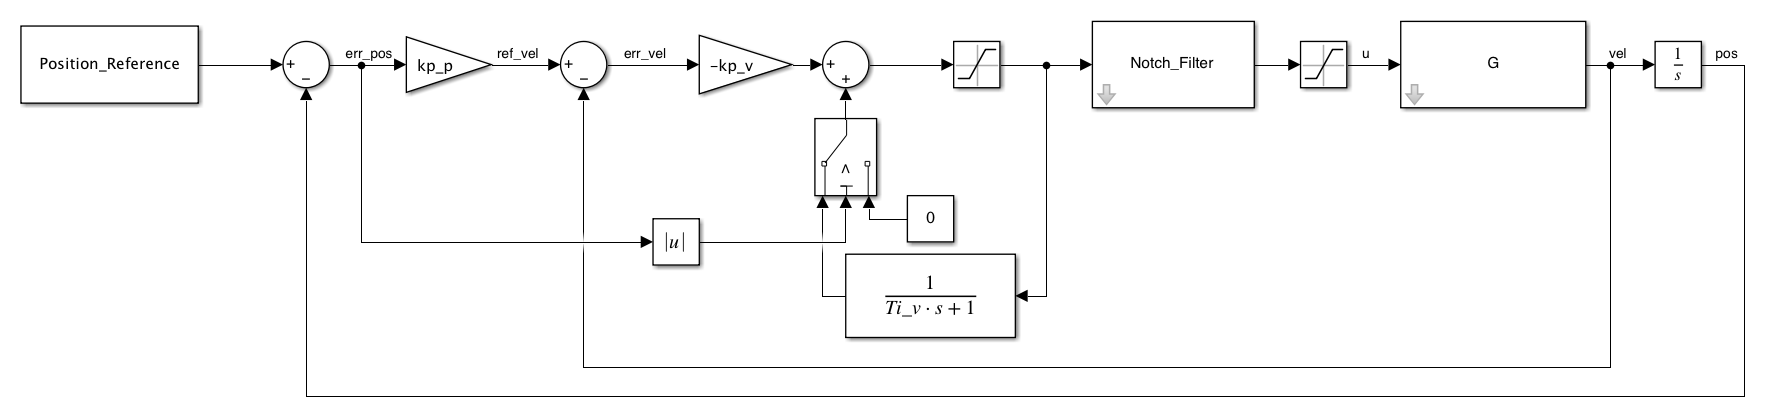
\includegraphics[width=0.8\textwidth]{1dof_P_scheme}
	\caption{Closed-loop block scheme}
\end{figure*}

\paragraph{Tuning and simulation}
The inner loop controls the speed, whereas the outer one the position. For the first loop, it is used the same PI structure as the previous section, while the position is regulated by using a proportional controller. It is important to remark that the cutting frequency of the position and the speed one must be far enough (about one decade) to ensure the frequency decoupling of the two loops. As consequence, if it is maintained the cutting frequency of the speed loop as decided before ($k_v=4.5$ that corresponds to a bandwidth of~$17\ rad/s$, as estimated in the sine-sweep in \cref{fig:sinesweep_PI_1dof}), a first possible solution is reached by setting the position cutting frequency equal to~$1.7\ rad/s$; however, this solution seems to be extremely slow (only simulation is shown in \cref{fig:P1dof_step}, without experimental data). \\

To overcome this problem, the ratio between the speed cutting frequency and the position one can be pushed up to~$20\ \%$. In this scenario, the proportional gain can be fixed in order to have a higher bandwidth: firstly~$\omega_{c,p} = 2\ rad/s$ and, then, also~$\omega_{c,p} = 3.5\ rad/s$.
In \cref{fig:P1dof_step} all these three cases are compared.
\begin{figure*}[h]
	\centering
	\begin{subfigure}{0.45\columnwidth}
		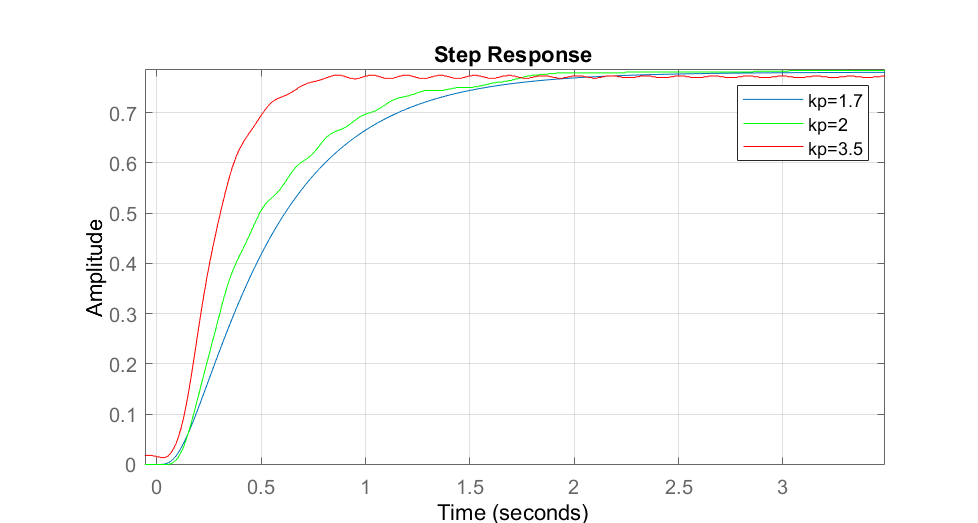
\includegraphics[width=\textwidth]{1dof_P_comparison}
		\subcaption{Closed-loop step responses}
		\label{fig:P1dof_step}
	\end{subfigure}
	\begin{subfigure}{0.45\columnwidth}
		\begin{tabular}{|c|ccc|}
			\hline
			Results\footnote{Gain margin~$G_m$ and phase margin~$\phi_m$ are obtained theoretically by means of MATLAB. Instead, settling time~$T_s$ is measured through data collected at the laboratory.} & $\omega_{c,p}=1.7$ & $\omega_{c,p}=2$ & $\omega_{c,p}=3.5$ \\
			\hline
			$G_m\ [dB]$ & $23.2$ & $21.7$ & $16.9$ \\
			$\phi_m\ [deg]$ & $78.0$ & $76.0$ & $63.3$ \\
			\hline
			$T_s\ [s]$ & $2.30$ & $1.80$ & $0.75$ \\
			\hline
		\end{tabular}
	\end{subfigure}
	\caption{Comparisons between $w_{c,p}=1.7$, $w_{c,p}=2$ and $w_{c,p}=3.5$ cases}
	\label{fig:Bode and Step P 1dof comparison}
\end{figure*}
The last case is certainly the fastest one, so it is considered the best solution reached so far. \\
However, small oscillations occur after the end of the transient; initially, we thought that those were caused by the coupling of speed and position control loops: this suggested us to not speed up the controller with a higher proportional gain, in order to avoid greater oscillations. Spending more time thinking about this problem allowed us to deduce that the previous hypothesis was wrong. A more reasonable explanation attributes the cause of these oscillation to the switch of integrator in the inner loop; so actually, following this reasoning, a faster system could have been obtained. \\

Definitely, the~$\omega_{c,p} = 3.5\ rad/s$ tuning has been chosen, at that time, as the best solution. Results are in \cref{fig:Pos_1dof_3.5}.
\begin{figure*}[h]
	\centering
	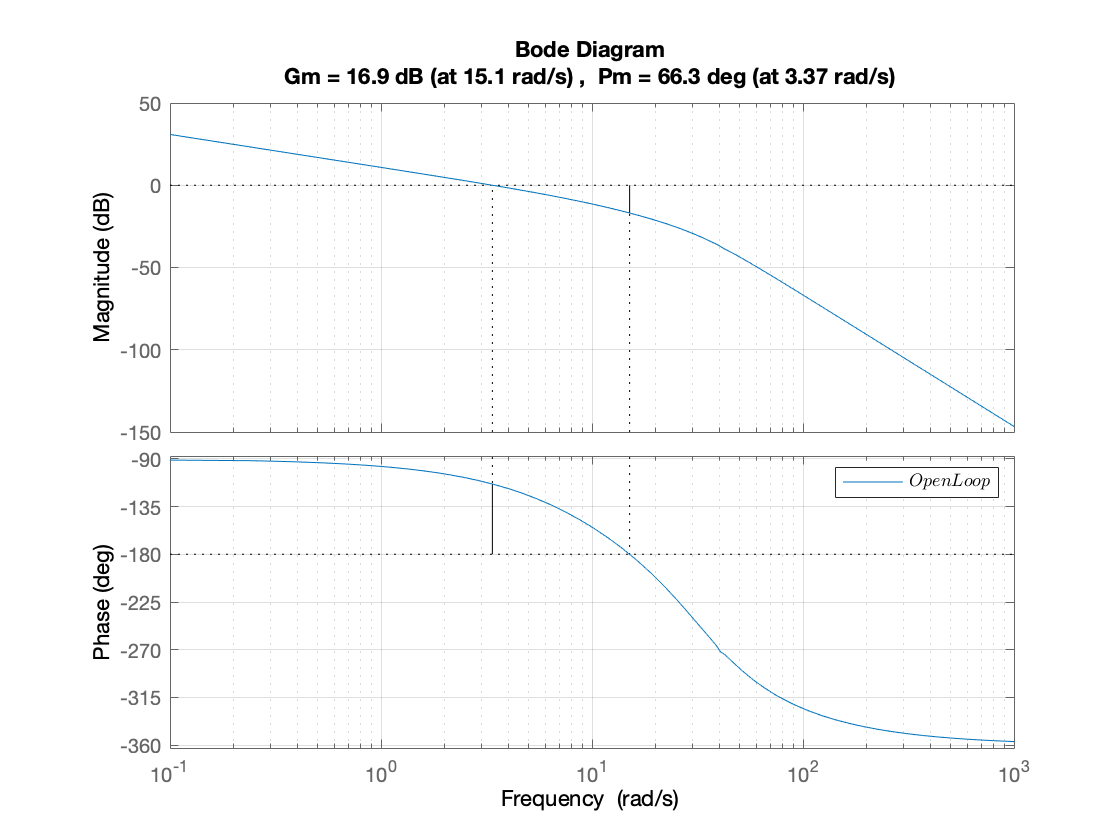
\includegraphics[width=0.4\textwidth]{1_bode3.5}
	\caption{Position control loop with  $w_{c,p}=3.5\ rad/s$}
	\label{fig:Bode P 3.5}
\end{figure*}

\begin{figure*}[h]
	\centering
	\begin{subfigure}{0.45\columnwidth}
		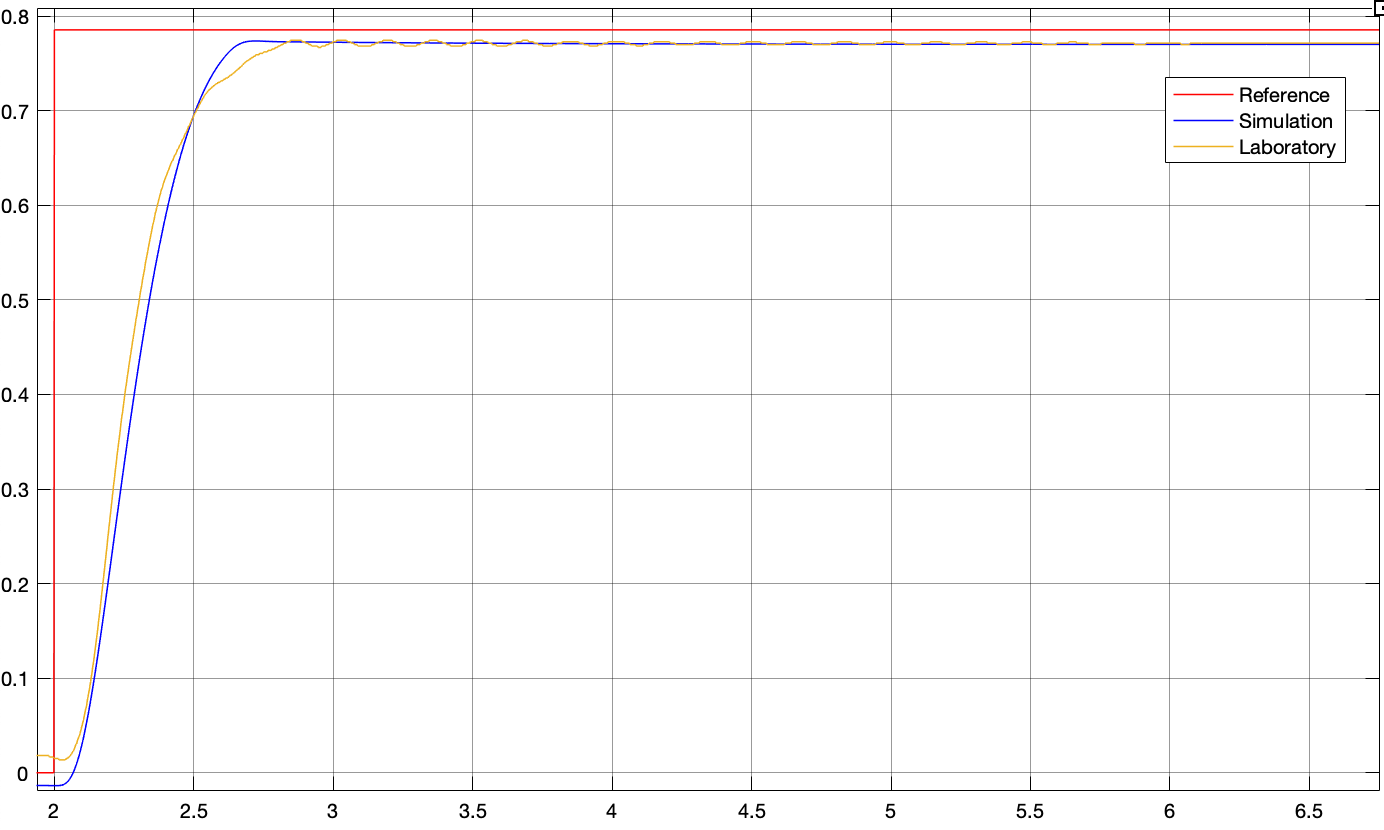
\includegraphics[scale=0.3]{pos_1_dof}
		\caption{Position}
	\end{subfigure}
	\begin{subfigure}{0.45\columnwidth}
		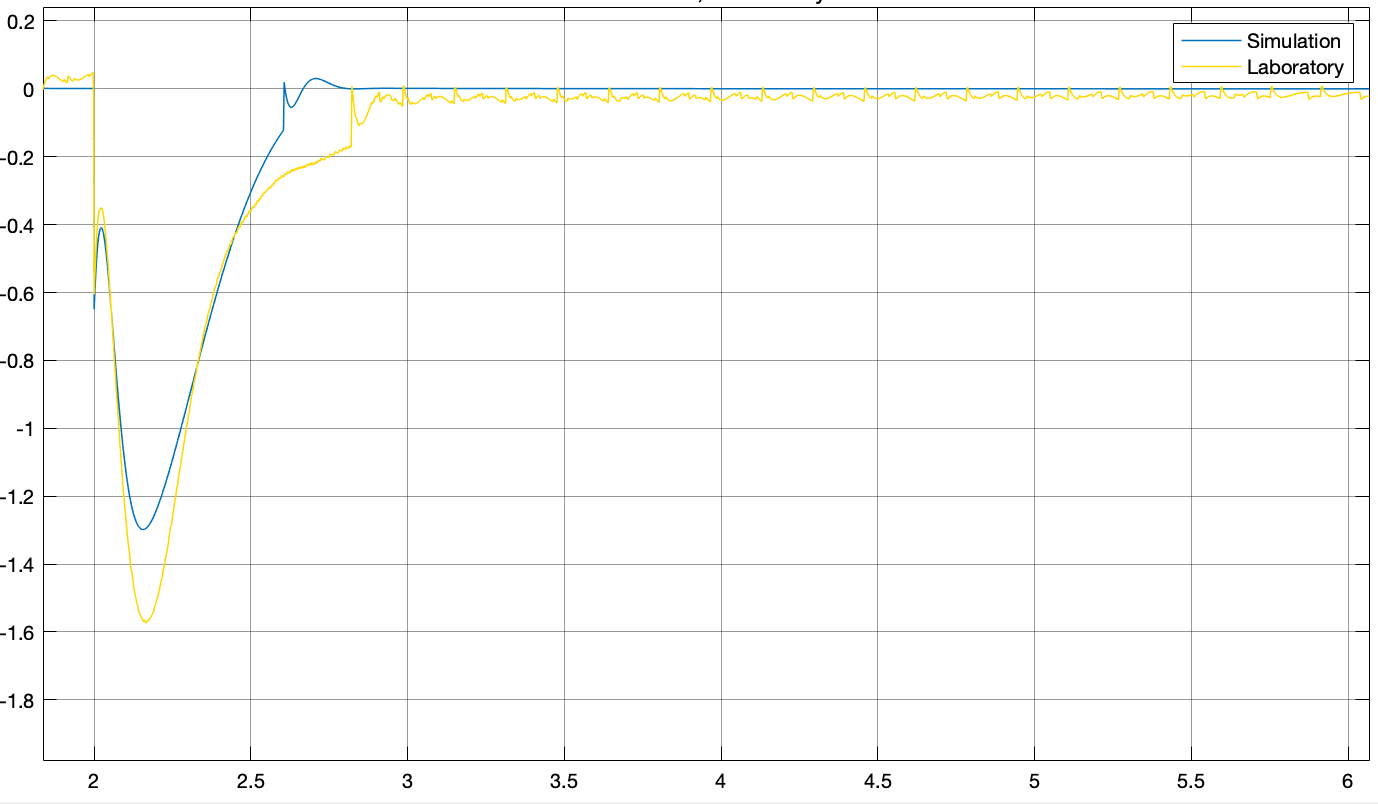
\includegraphics[scale=0.3]{volt_1_dof}
		\caption{Voltage}
	\end{subfigure}
	\caption{Step response with $\omega_{c,p}=3.5$}
	\label{fig:Pos_1dof_3.5}
\end{figure*}

\newpage
Due to the friction, the position reached by the mass is not exactly the reference one. The controller integrates this small error and the control input raises slowly. Since the static friction coefficient is higher than the dynamic one, the load will move only after a few seconds, during which the controller has kept integrating the error asking for an increasing control action.
Once that the input is large enough to counteract the static friction, the load moves and the friction drops, making the applied control input stronger than what needed. The result is that the load moves over the reference, generating an error that is even bigger than the original one.
For the above-mentioned reasons, a logic switch has been implemented. Its purpose is that of deactivate the integrative action of the inner loop whenever the position error is smaller than a threshold equal to~$0.85 \degree$. On the other hand, it is not possible to zero error at steady state since only the proportional action is in place.
\begin{figure*}[h]
	\centering
	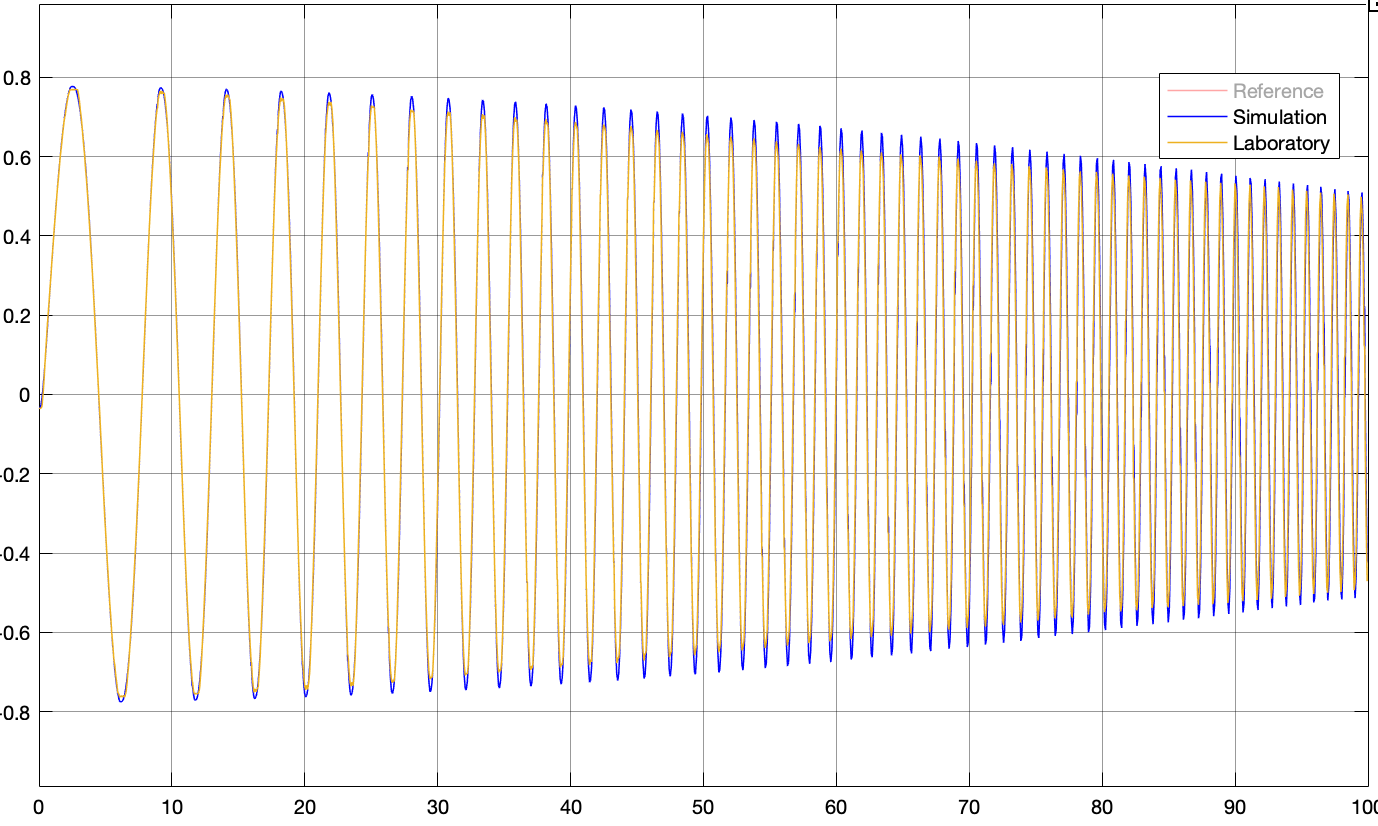
\includegraphics[scale=0.2]{sine_pos_1dof}
	\caption{Sine-sweep experiment from $0.1\ Hz$ to $1\ Hz$ in $100\ s$}
	\label{fig:sinesweep_pos_1dof}
\end{figure*}

Also in this case, a sine-sweep experiment is performed to estimate the bandwidth of the closed loop system. The simulation and laboratory data are really close and the cutting frequency is around~$5.5\ rad/s$ for the simulated system and~$4.5\ rad/s$ for the real system.
\newpage
\section{\twodof\ system}
Consider the transfer function from voltage to the second mass speed:
\[
G_{v,\dot{\theta}_2}(s)=
\frac{-1.293 \cdot 10^{8}}{s^5+40.9s^{4}+4833s^{3}+1.686 \cdot 10^{5} s^{3}+3.327 \cdot 10^{6} s+7.355 \cdot 10^{7}}
\]

\begin{figure*}[h]
	\centering
	\begin{subfigure}{0.4\columnwidth}
		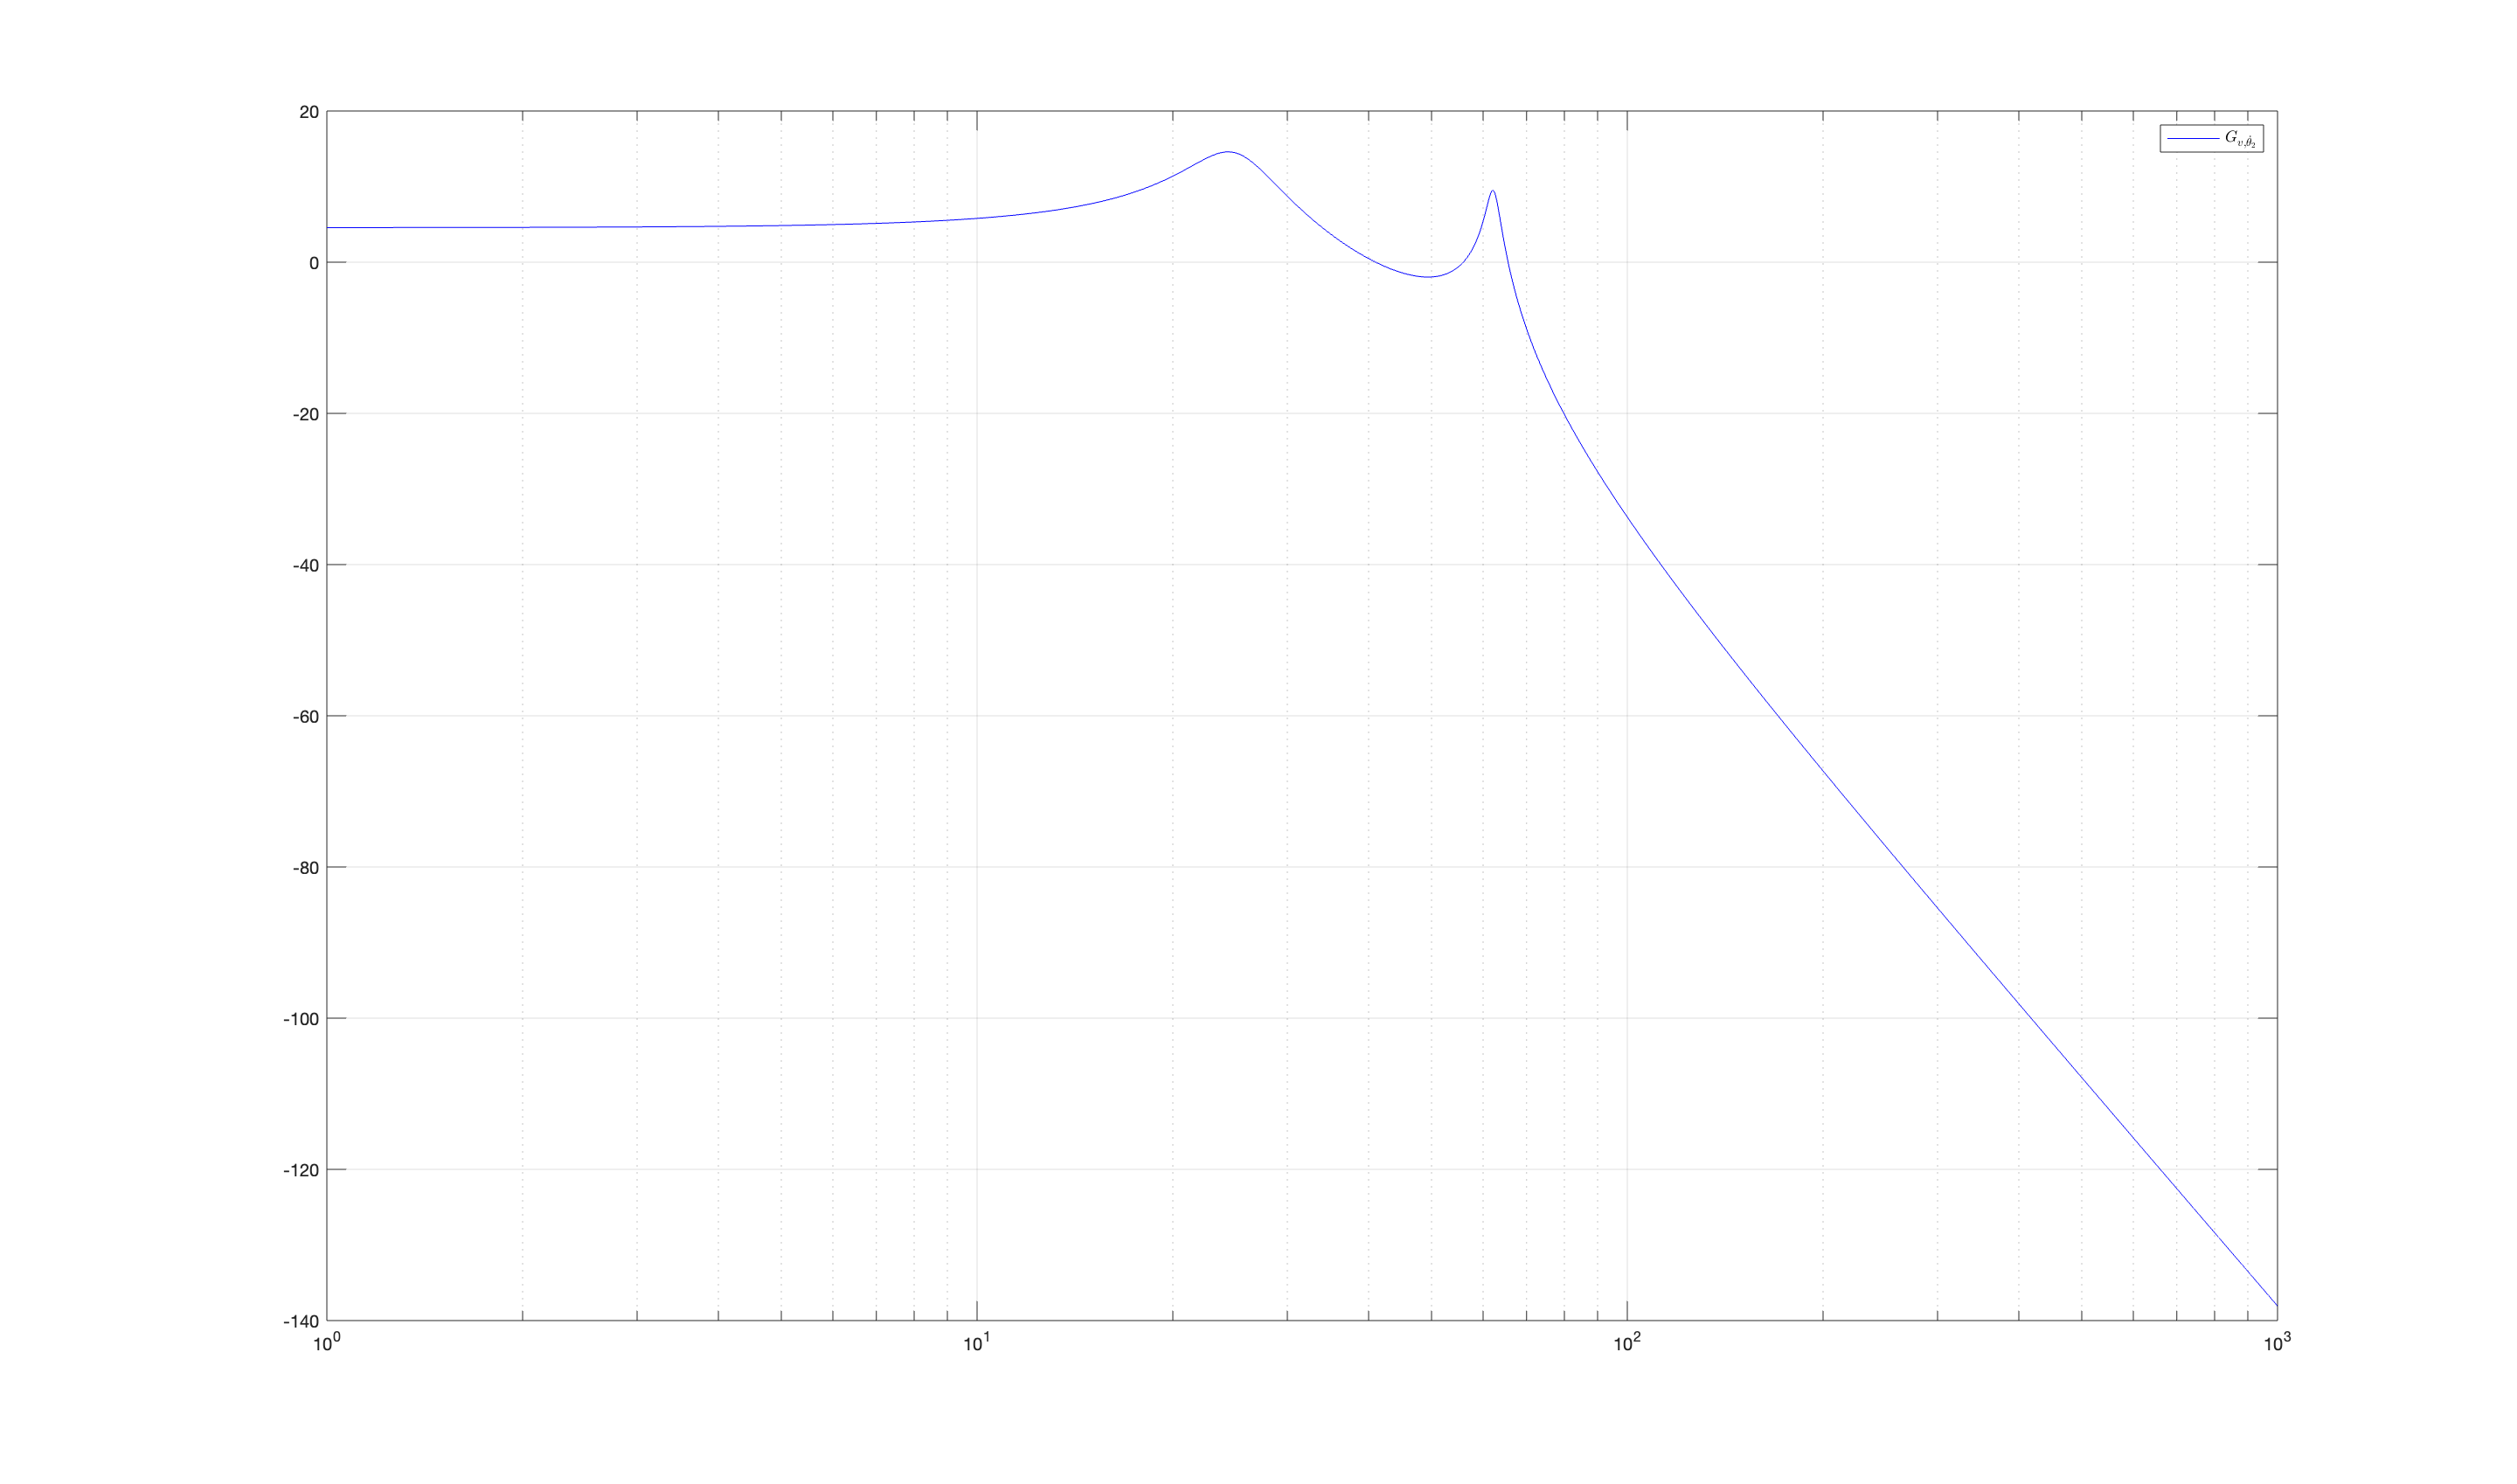
\includegraphics[width=\textwidth]{1_bodeG2}
	\end{subfigure}
	\begin{subfigure}{0.4\columnwidth}
		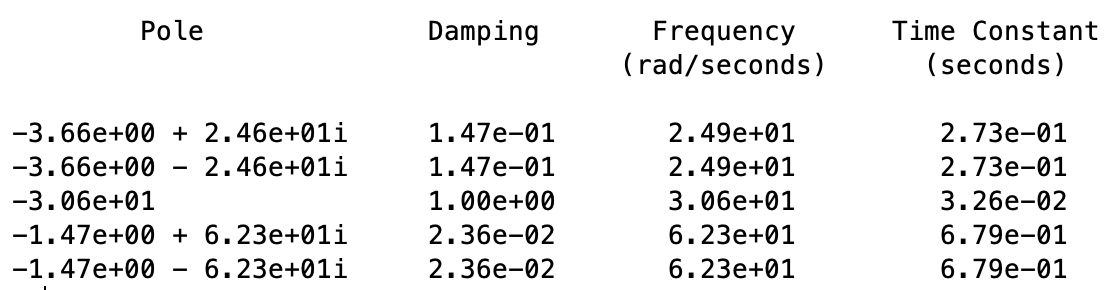
\includegraphics[width=\textwidth]{1_poleG2}
	\end{subfigure}
	\caption{G(s)}
	\label{fig:G(s)2dof}
\end{figure*}

As it is possible to notice in \cref{fig:G(s)2dof}, there are now two couples of complex conjugated poles with low damping coefficient. A similar solution to the \onedof\ problem has been applied, it is used a notch filter to delete these poles and substitute them with a couple of complex conjugated poles, this time at frequency~$100\ rad/s$ and a damping coefficient equal to~$0.72$. The reason why it has been decided to postpone the poles frequency instead of using the original one is explain in the speed control loop section.


\begin{figure*}[h]
	\centering
	\begin{subfigure}{0.45\columnwidth}
		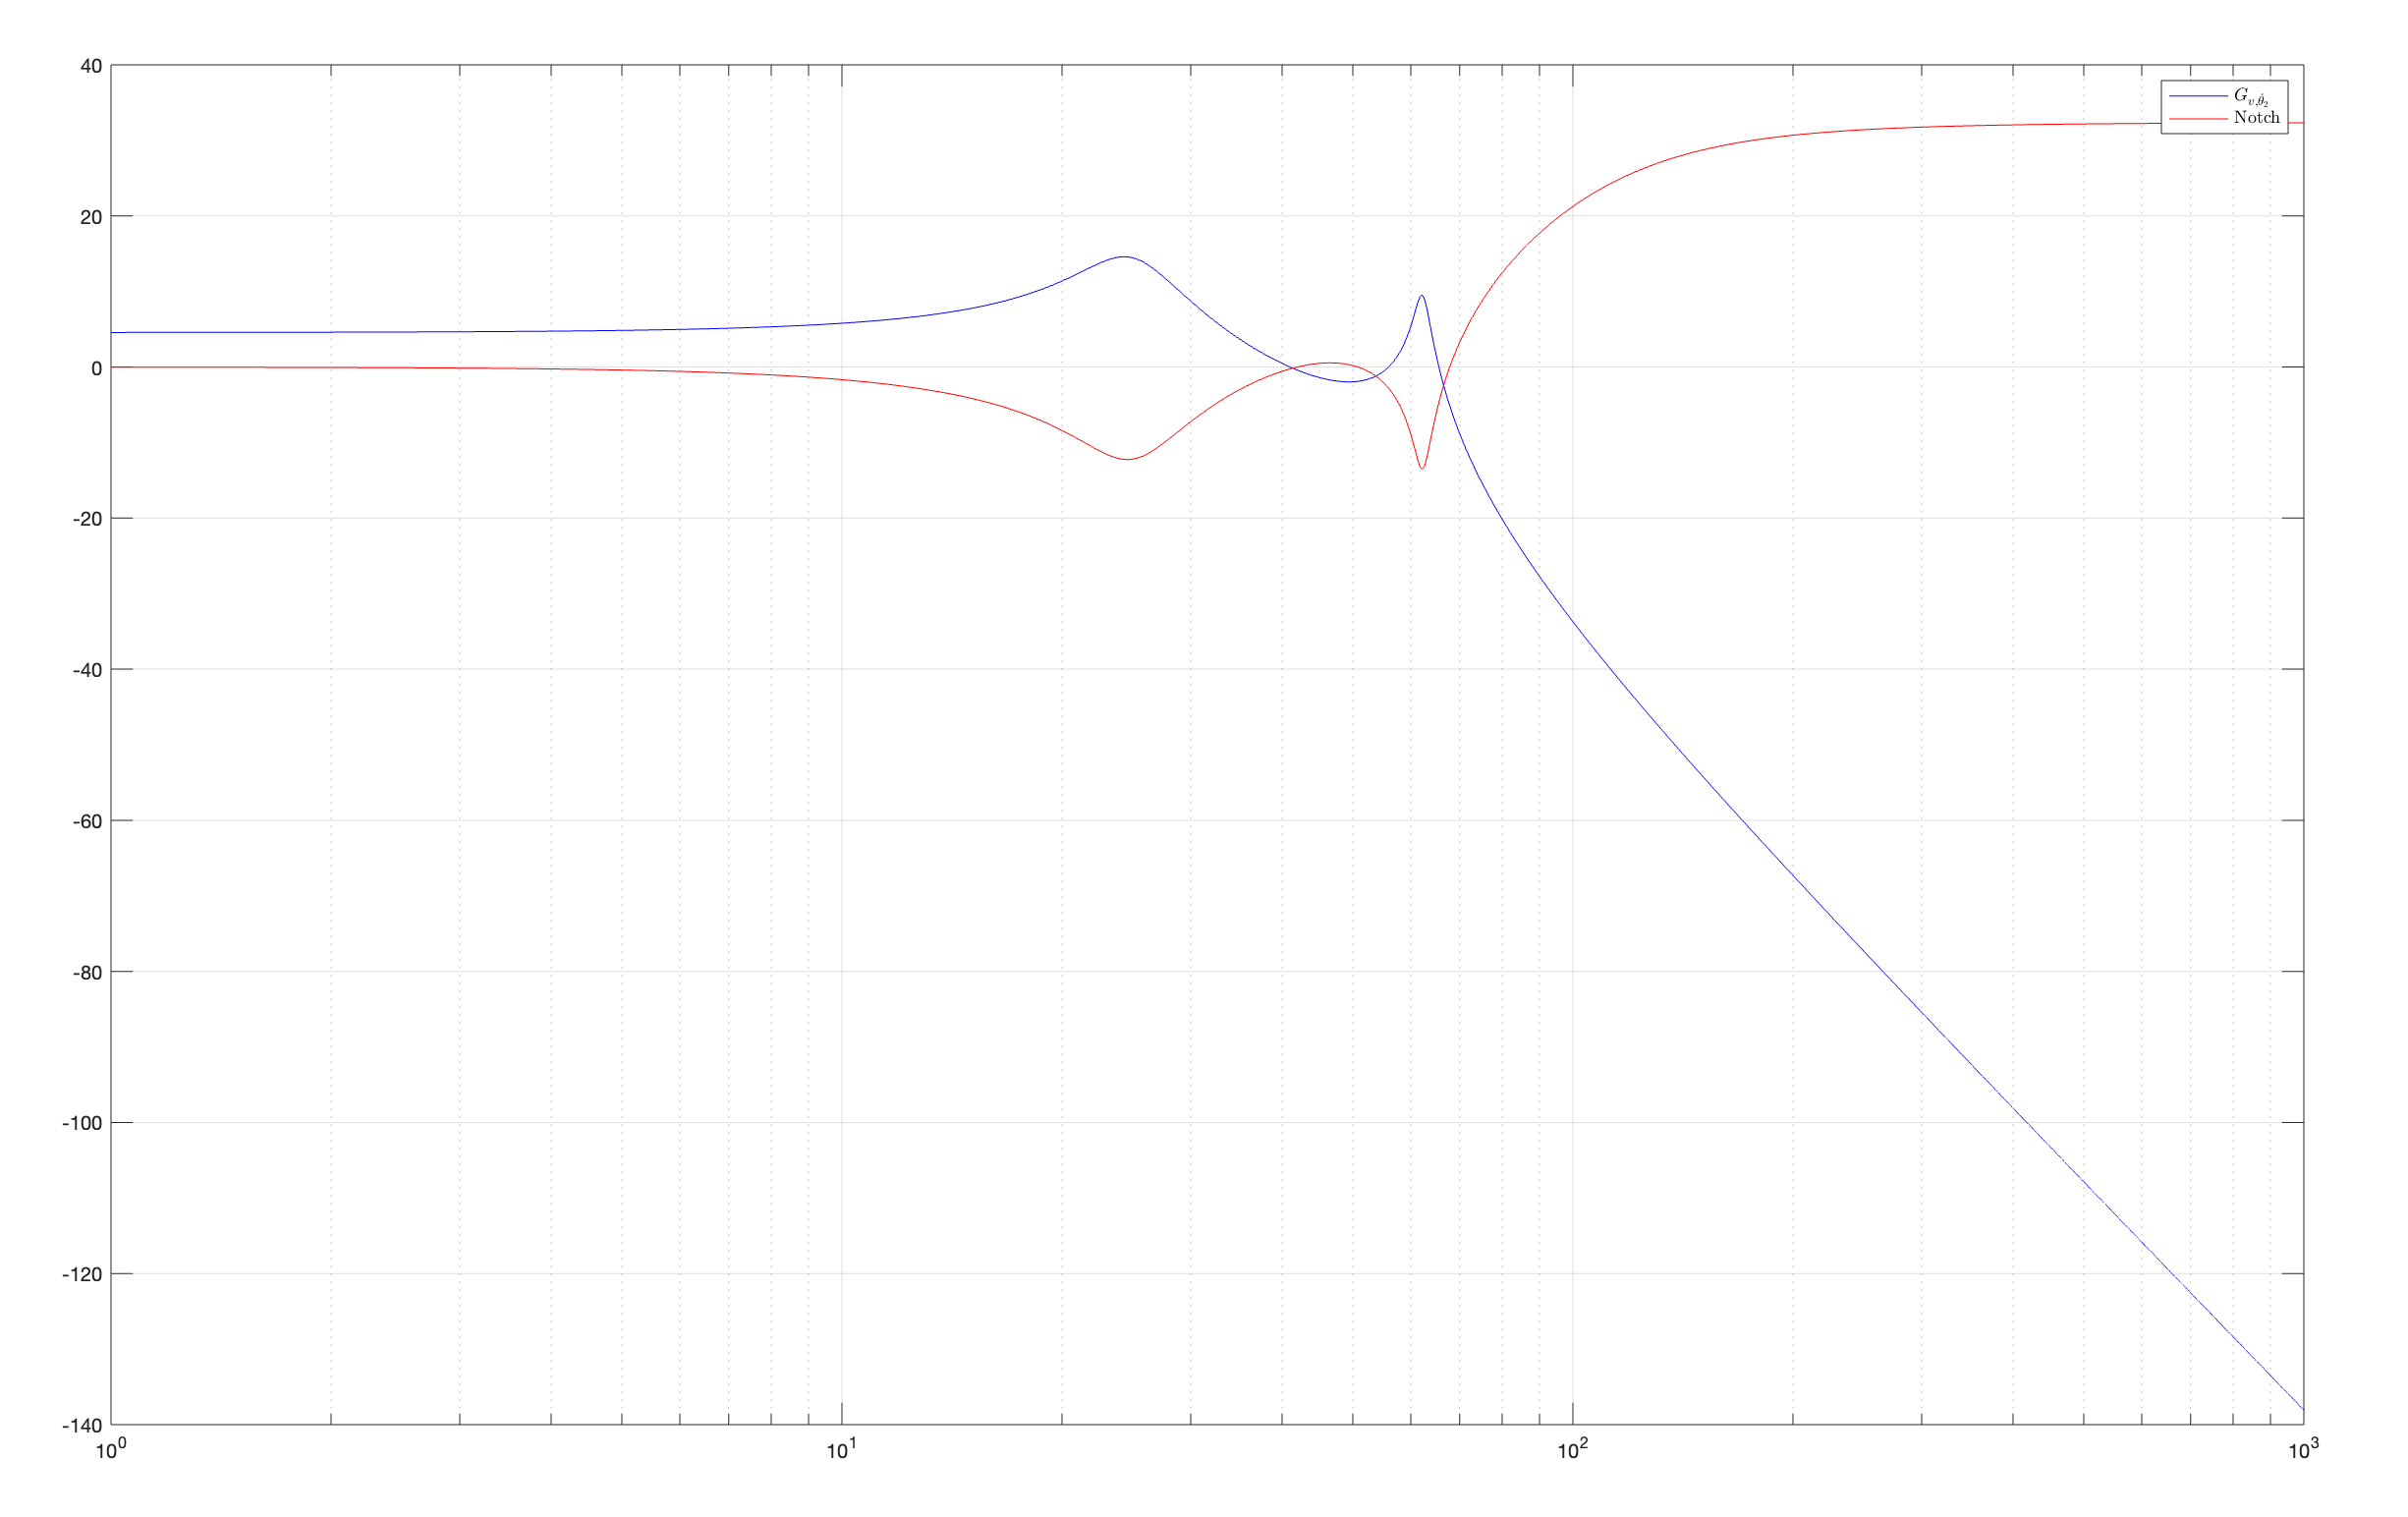
\includegraphics[width=\textwidth]{1Nf_G2}
		\subcaption{$N_f(s)$ and $G(s)$}
		\label{fig:Notch Filter2}
	\end{subfigure}
	\begin{subfigure}{0.45\columnwidth}
		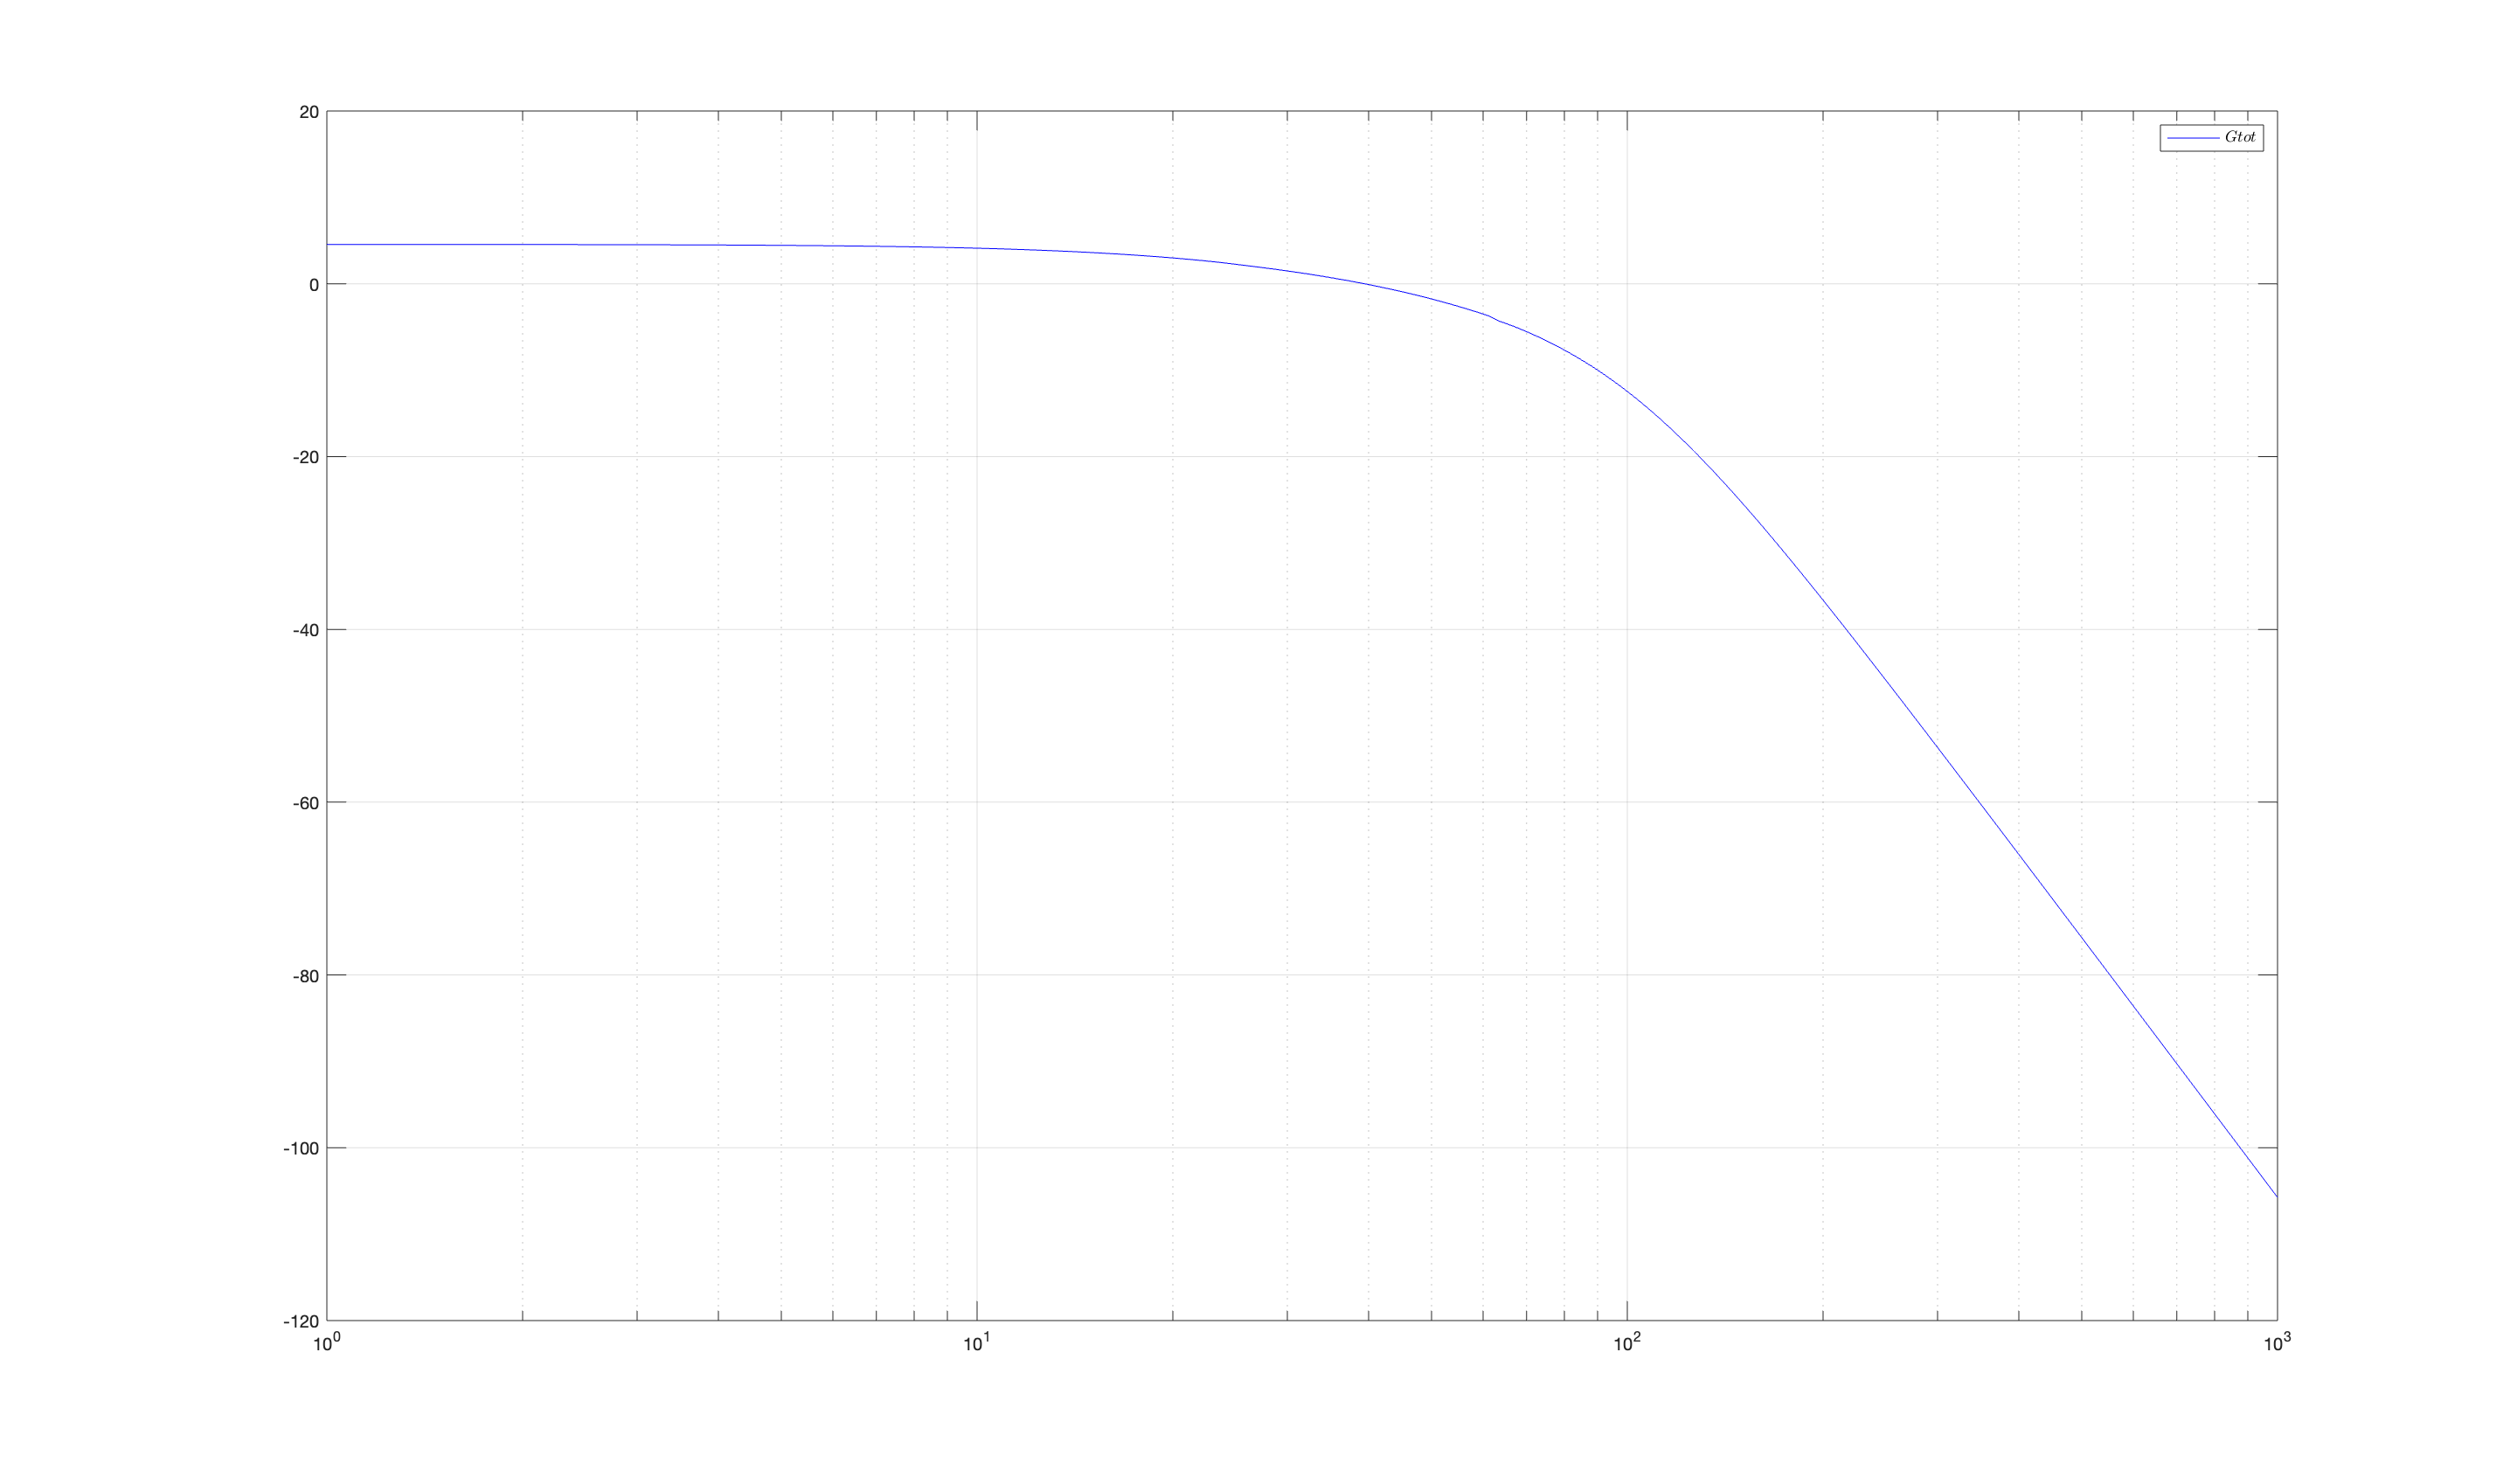
\includegraphics[width=\textwidth]{1_G2tot}
		\subcaption{$G_{tot}(s)$}
		\label{fig:Plant G(s) with Notch Filter2}
	\end{subfigure}
	\caption{Plant $G(s)$ with Notch Filter $N_f(s)$: $G_{tot}$(s)}
\end{figure*}


Applying the notch filter represented in \cref{fig:Notch Filter2}, the controller sees the plant~$G_{tot}(s)$ of \cref{fig:Plant G(s) with Notch Filter2}.

\newpage 
\subsection{Speed Control Loop}
The controller structure is the PI, enriched with an anti-wind-up structure; as before, the zero of the PI controller cancels out the real pole at~$30.6\ rad/s$.
\[
R(s)=-k_v
\frac{\frac{s}{30.6}+1}{s}
\]

As noticed in the \onedof~case, there are some periodic oscillations due to a change of the dynamic friction along the revolution of the masses. Right now the amplitude of these disturbances cannot be neglected anymore and a solution to attenuate them as much as possible needs to be found. In order to enhance the disturbance rejection, a~$w_{c,v}$ high enough to obtain a large bandwidth is required. On the other hand, it is not possible to set it at high frequencies, otherwise the phase margin would decrease dramatically. A good trade-off is imposing~$k_v=5$.
 In order to design the right controller, in the simulation scheme it has been added a disturbance acting on both torques (\textit{mass1} and \textit{mass2}) with fixed amplitude at~$0.005$ and frequency equal to the masses speed to simulate this change of the dynamic friction during the revolution.
\begin{figure*}[h]
	\centering
	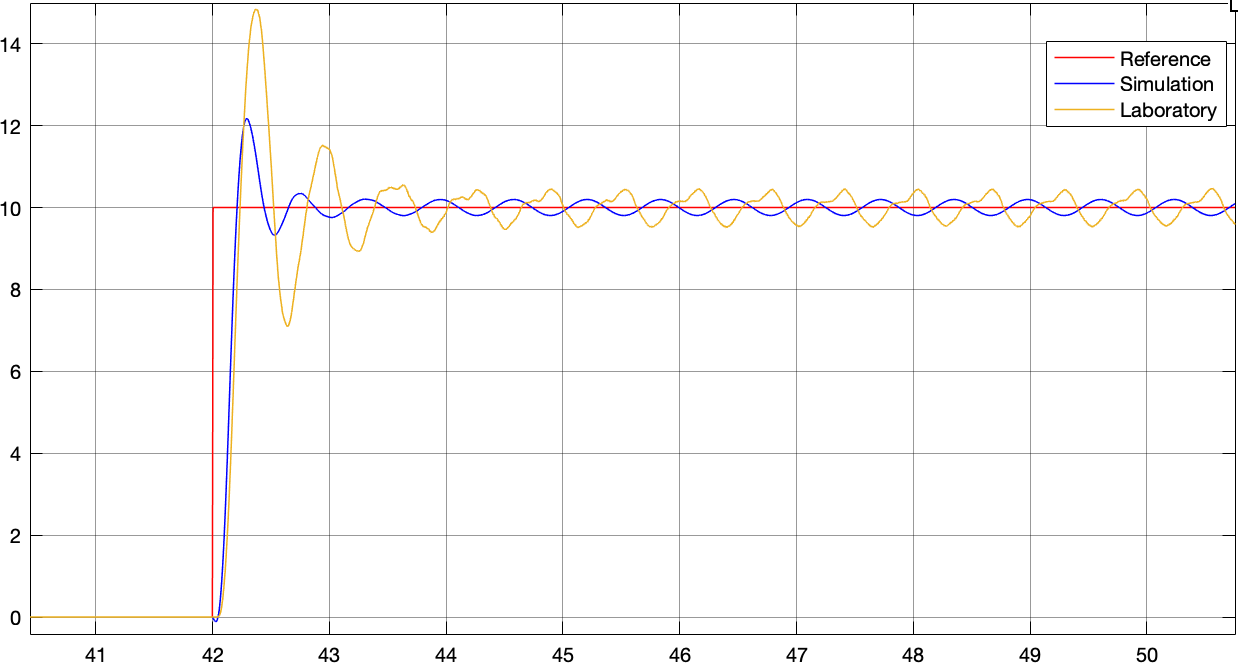
\includegraphics[scale=0.4]{step10_noPF}
	\caption{Step response with $k_v=5 $}
	\label{fig:step10_noPF}
\end{figure*}

This solution is far to be acceptable due to its high oscillations during the transient. To keep large enough the bandwidth, it has been decided not to anticipate the~$w_{c,v}$, but to build a low-pass pre-filter on the reference signal with cutting frequency at~$7\ rad/s$. Thanks to this solution, the closed loop system will not be excited by high frequencies and two other positive effects appear: no oscillations during the transient and rejection of the resonances identification uncertainties. Indeed, the amplitudes of the oscillations at steady state are decreased and now can be considered acceptable. 

\newpage
\begin{figure*}[h]
	\centering
\begin{subfigure}{0.4\columnwidth}
	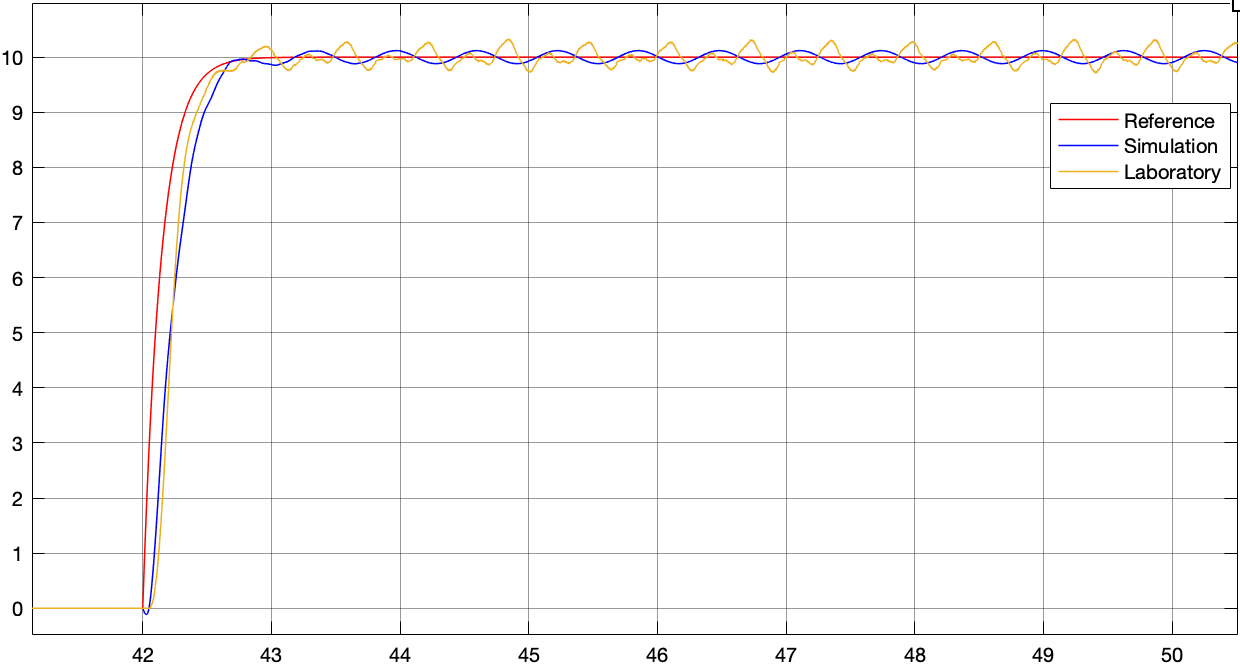
\includegraphics[width=\textwidth]{step10}
	\subcaption{Step $10\ rad/s$}
\end{subfigure}
\begin{subfigure}{0.4\columnwidth}
	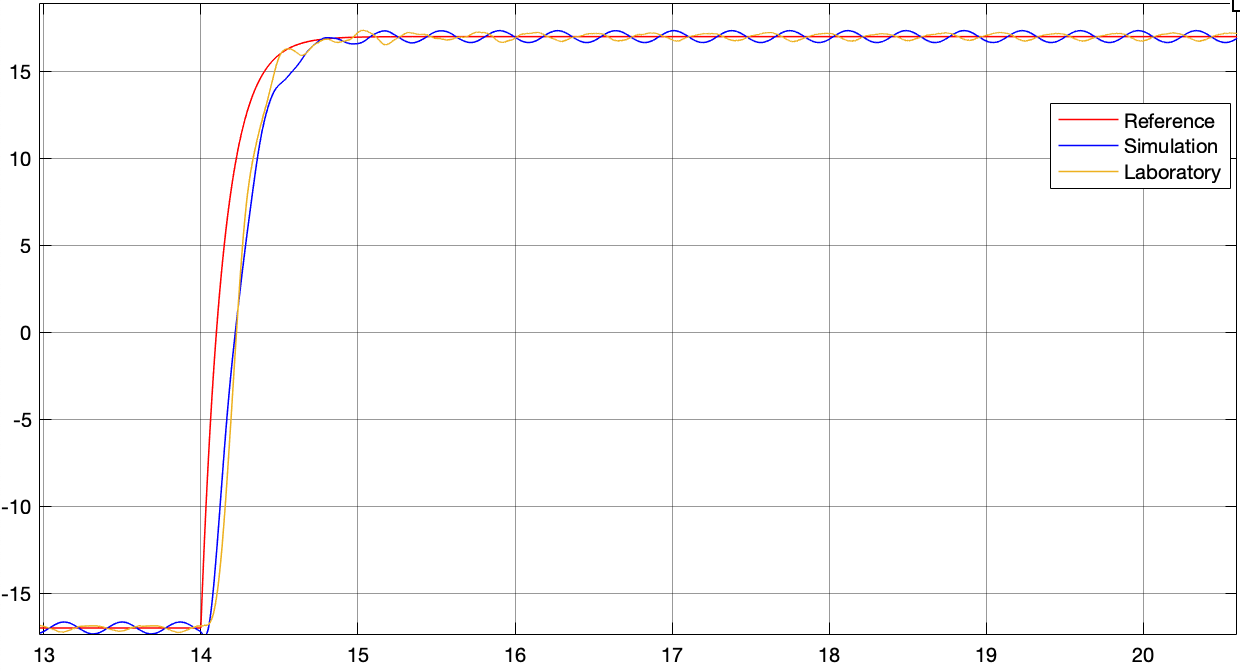
\includegraphics[width=\textwidth]{step17}
	\subcaption{Step $17\ rad/s$}
\end{subfigure}
\begin{subfigure}{0.4\columnwidth}
	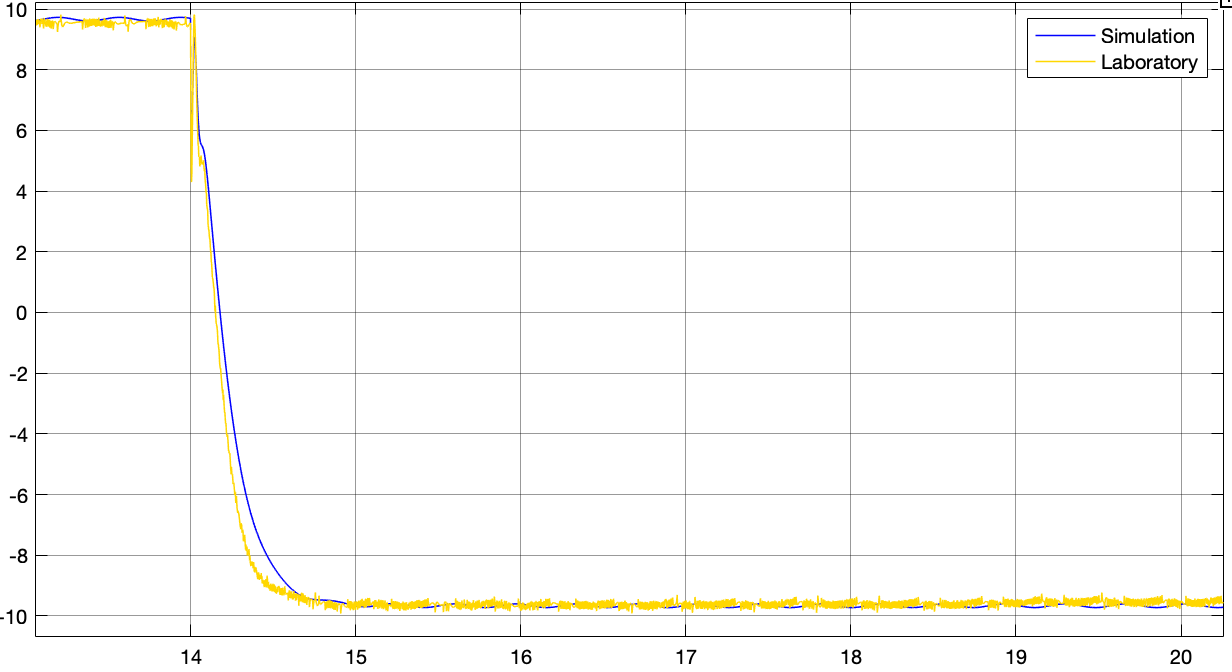
\includegraphics[width=\textwidth]{volt17}
	\subcaption{Voltage related to a step of $17\ rad/s$}
\end{subfigure}
\caption{Speed control loop with $k_v=5$ with low-pass pre-filter}
\label{fig:PI_with_5}
\end{figure*}

As it is possible to notice in figure \ref{fig:PI_with_5}, the simulation and laboratory data are really close during the transient and the voltage never saturates. This solution satisfies the requirements. The \cref{fig:sinesweep_speed_2dof} shows the response to a sinesweep without applying the pre-filter to the reference.  This is useful to understand the mismatch between the simulation and the real system in the range of frequency from 1 Hz to 10 Hz.

\begin{figure*}[h]
	\centering
	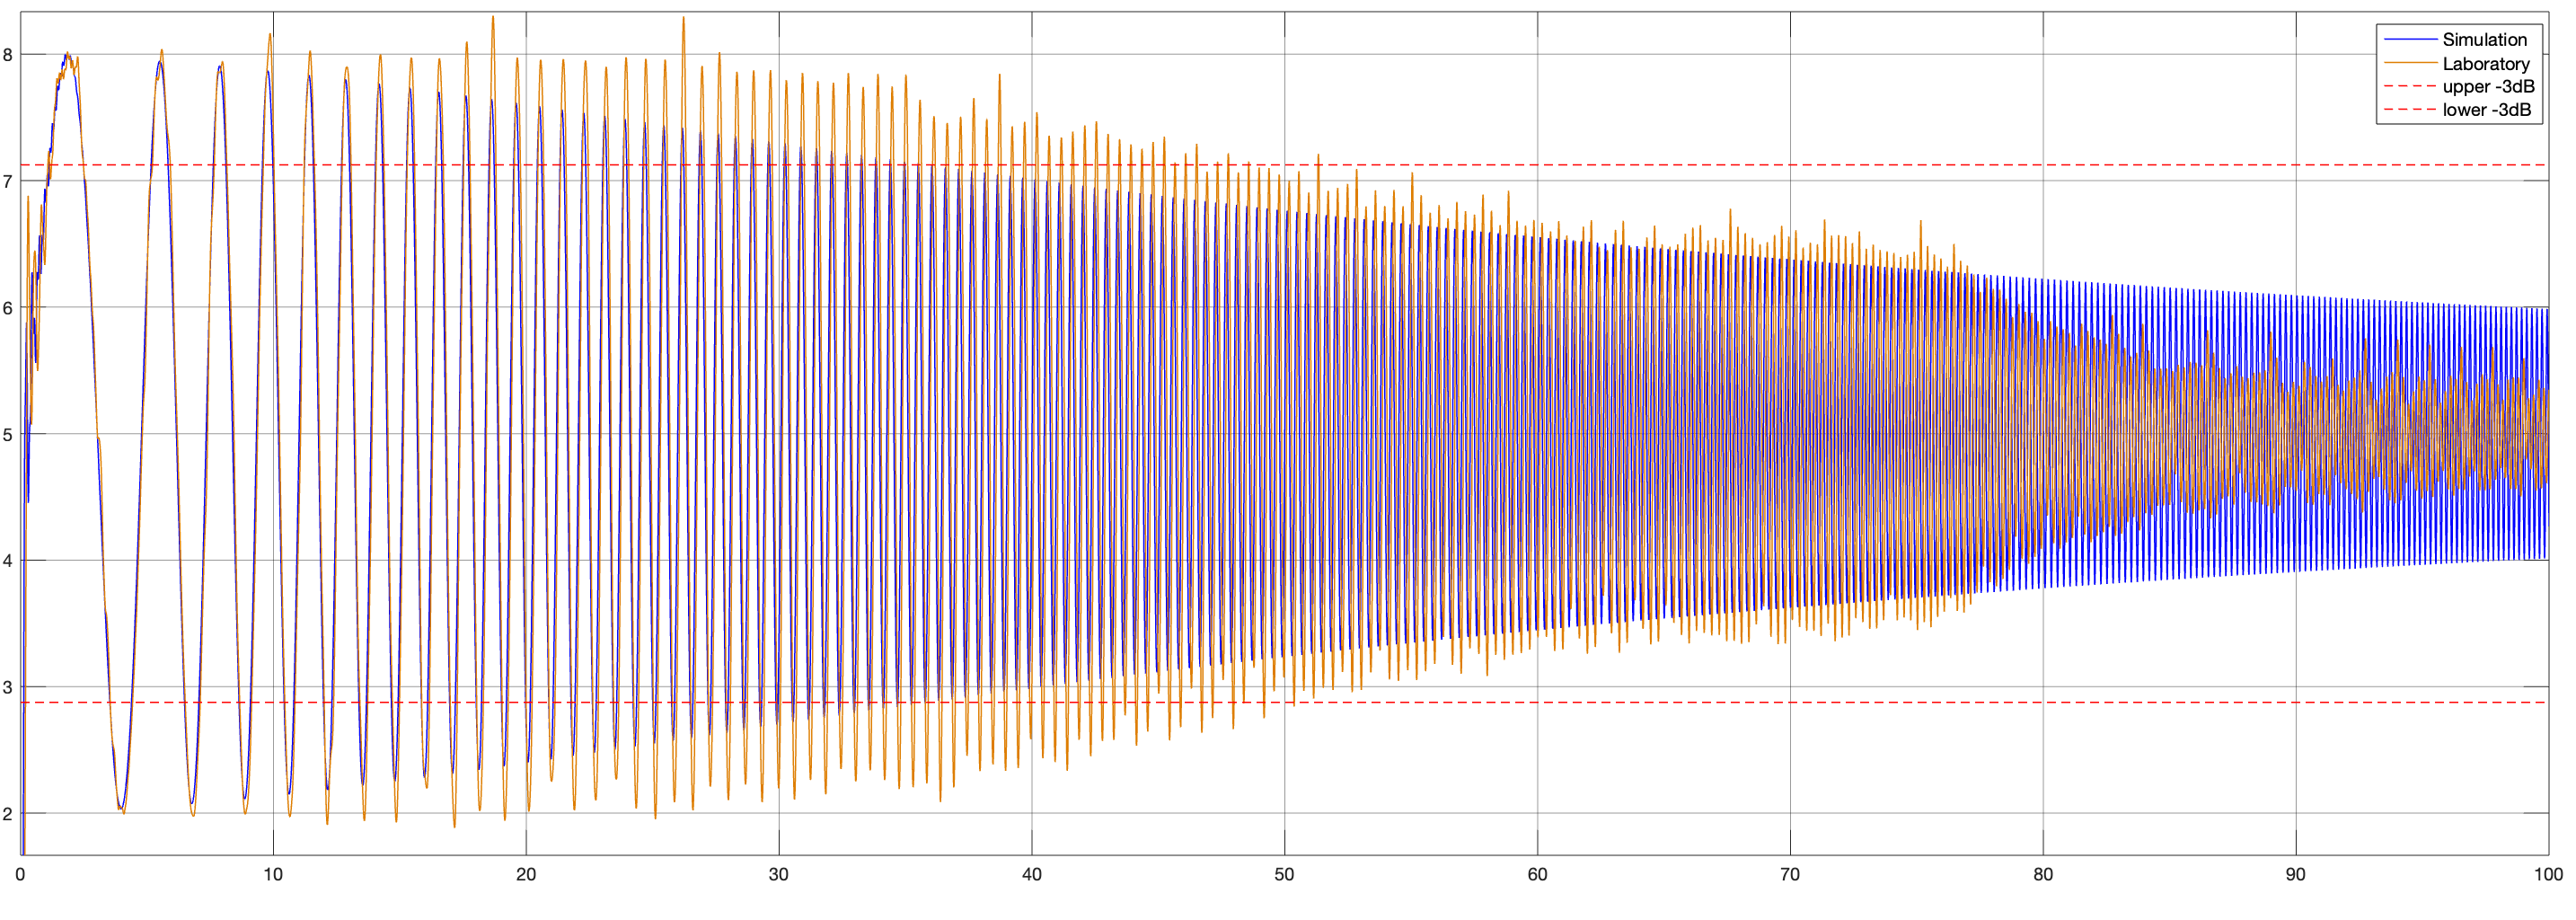
\includegraphics[scale=0.4]{sine_PI}
	\caption{Sineweep experiment from $1\ Hz$ to $10\ Hz$ in $100\ s$}
	\label{fig:sinesweep_speed_2dof}
\end{figure*}

From \cref{fig:sinesweep_speed_2dof}, it appears that the overall frequencial behavior of the simulation is similar to the real one. The main difference arises around 75 seconds that corresponds to a frequency around~$25\ rad/s$. At this frequency there is the first resonance peak of the plant. An explanation to this different behavior could be an overestimation of the damping coefficient. As consequence, the whole resonance peak has not been compensated completely and the sinesweep experiment shows it very well. \\

As it has been done for the \onedof\ system, the controllability range is tested with a ramp with decreasing low speed. In this case, the presence of small oscillations prevents the control the system at very low speed. For this reason the controllable speed belongs to two possible intervals: from~$-17\ rad/s$ to~$-0.5\ rad/s$ and from~$0.5\ rad/s$ to~$17\ rad/s$.
\begin{figure*}[h]
	\centering
	\begin{subfigure}{0.45\columnwidth}
		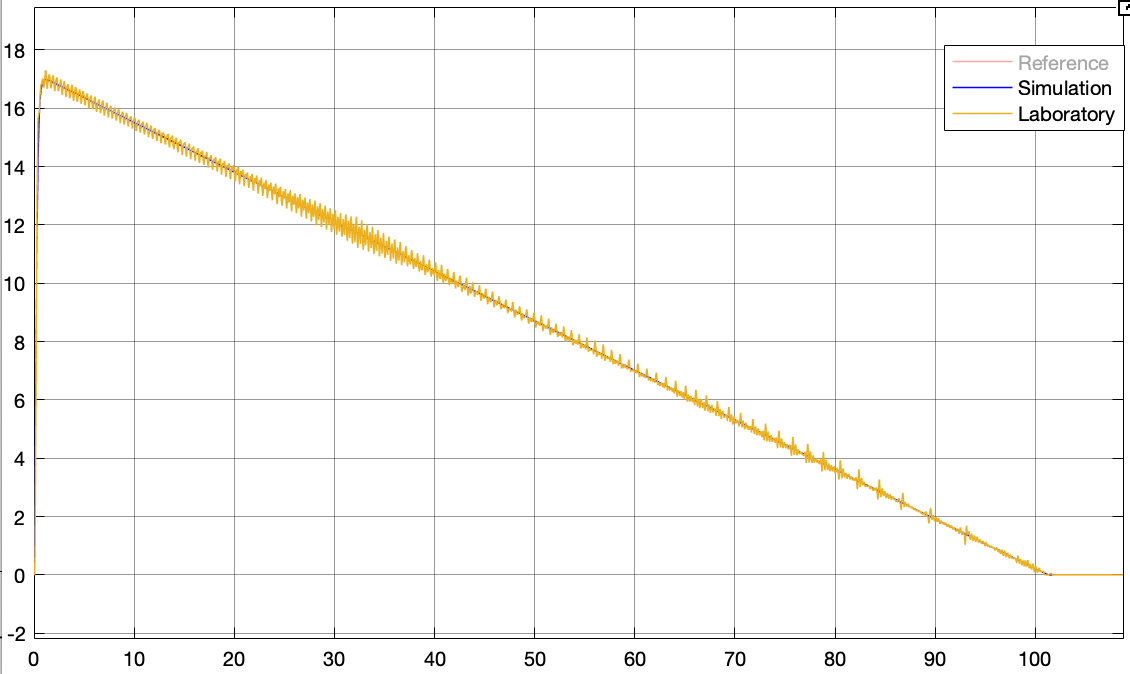
\includegraphics[width=\textwidth]{Ramp2dofa}
		\subcaption{Entire experiment}
	\end{subfigure}
	\begin{subfigure}{0.45\columnwidth}
		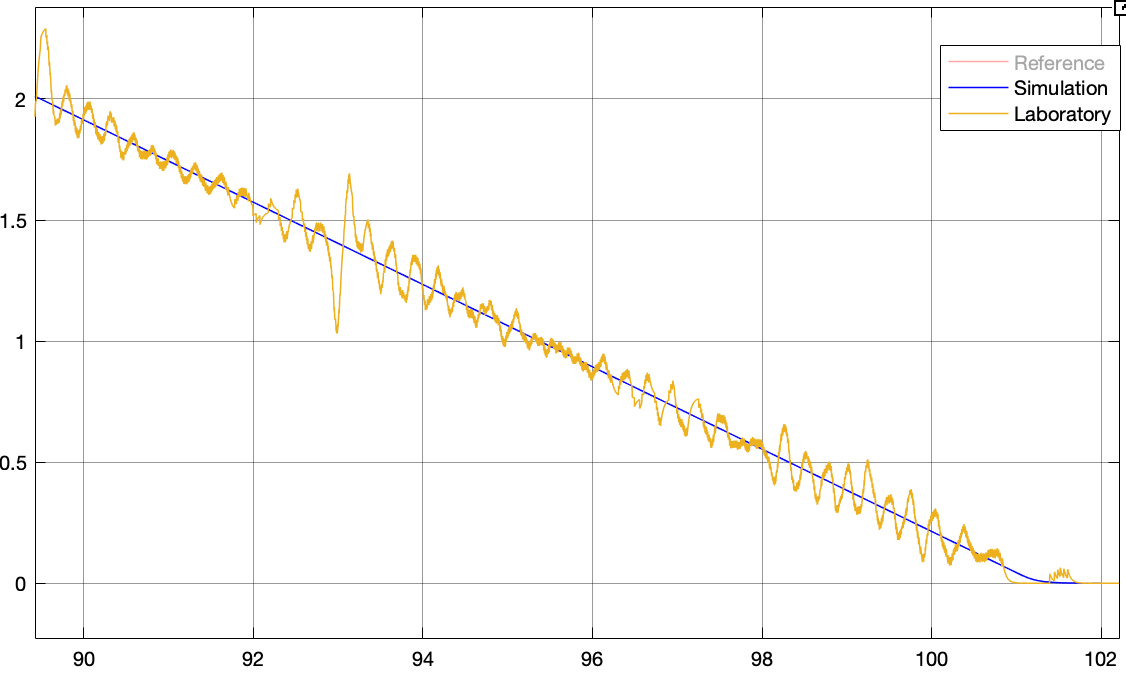
\includegraphics[width=\textwidth]{Ramp2dofb}
		\subcaption{Detail at low speed}
	\end{subfigure}

	\caption{Ramp experiment from $17\ rad/s$ to $0\ rad/s$ in $100\ s$}
	\label{fig:Ramp2dof}
\end{figure*}

\newpage
\subsection{Position Control Loop}

Following the same reasoning of the \onedof~case, a cascade control strategy is used. The low-pass filter solution in the inner loop is avoided, because of the change of the scheme: the reference signal does not enter directly to the speed closed loop, but the speed reference is now generated by the proportional gain of the outer loop. On the other hand, the inner loop without pre-filter leads to a more oscillating dynamic. 

\begin{figure*}[h]
	\centering
	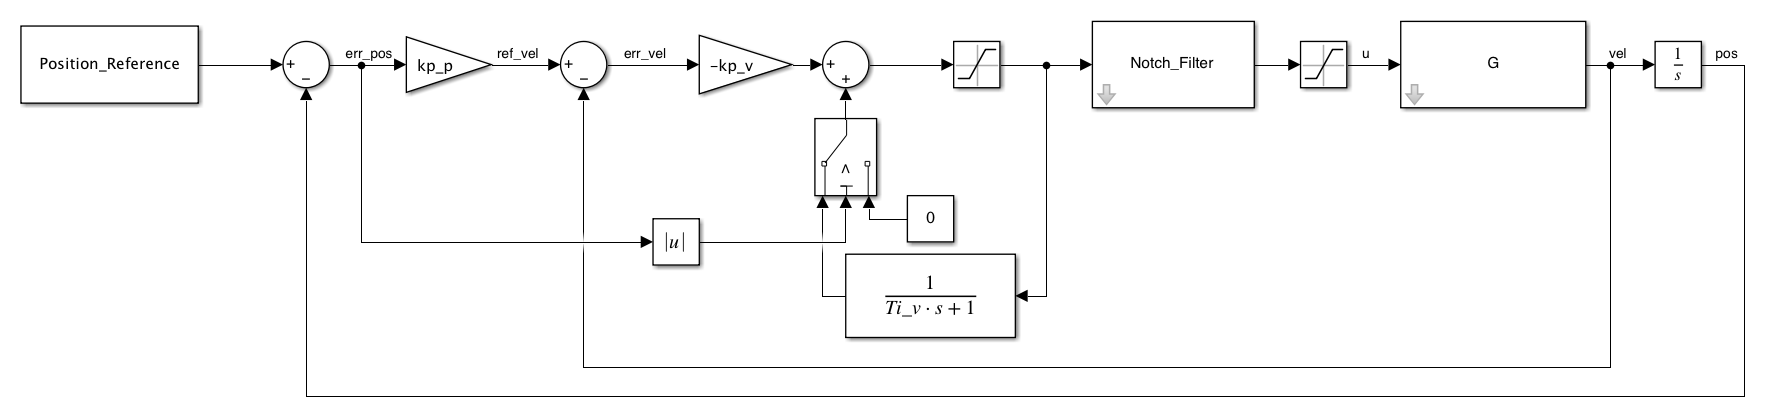
\includegraphics[width=0.8\textwidth]{1dof_P_scheme}
	\label{fig:Closed-loop block scheme2}
	\caption{Closed-loop block scheme}
\end{figure*}

A comparison between three different solutions is now provided:
\begin{itemize}
	\item $k_v=5 \ and\  \omega_{c,p}=3$
	\item $k_v=5 \  and\ \omega_{c,p}=2.5$
	\item $k_v=4 \ and\ \omega_{c,p}=2$
\end{itemize}

where $k_v$ represents the gain used to set the PI regulator of the inner loop, while $\omega_{c,p}$ is the bandwidth of the position loop. For the reason that each solution has a different $\omega_{c,p}$, from now on only $\omega_{c,p}$ will be used to distinguish them.

\begin{figure*}[h]
	\centering
	\begin{subfigure}{0.4\columnwidth}
		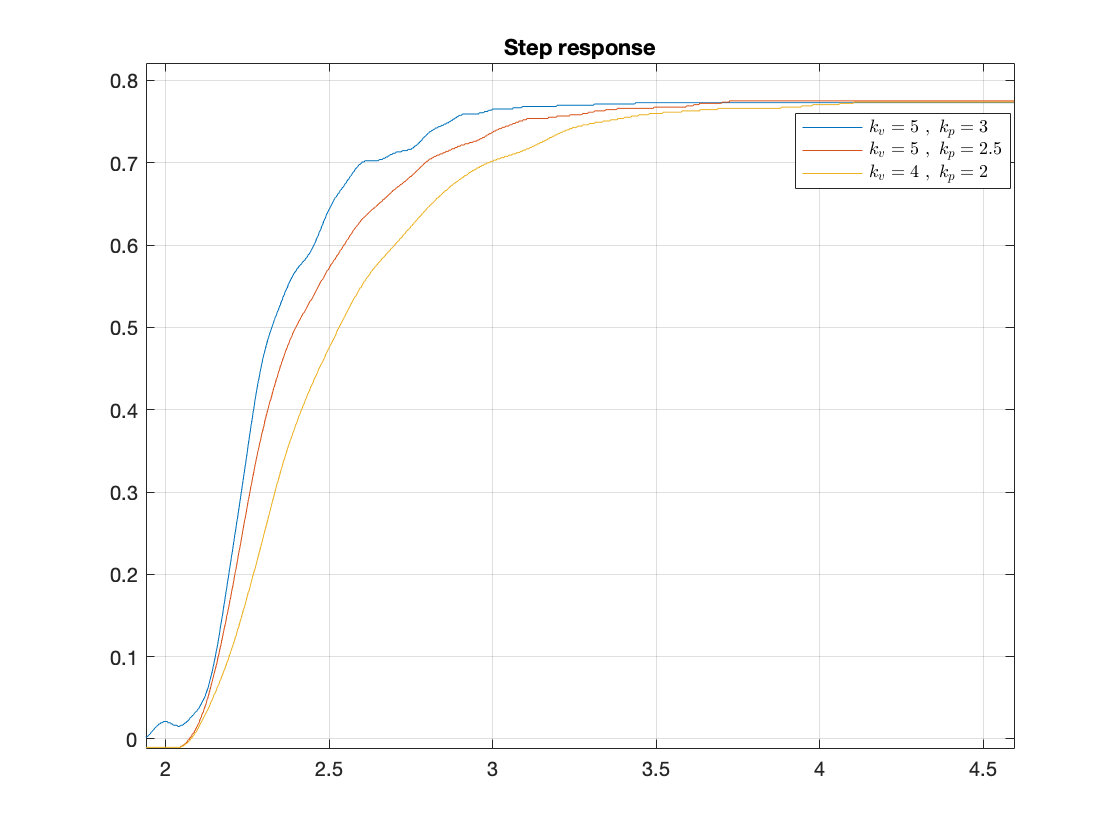
\includegraphics[width=\textwidth]{2dof_P_comparison}
		\subcaption{Closed-loop step responses}
		\label{fig:P2dof_step}
	\end{subfigure}
	\begin{subfigure}{0.4\columnwidth}
		\begin{tabular}{|c|ccc|}
			\hline
			Results\footnote{Gain margin~$G_m$ and phase margin~$\phi_m$ are obtained theoretically by means of MATLAB. Instead, settling time~$T_s$ is measured through data collected at the laboratory.} & $\omega_{c,p}=3$ & $\omega_{c,p}=2.5$ & $\omega_{c,p}=2$ \\
			\hline
			$G_m\ [dB]$ & $20.4$ & $22$ & $24.1$ \\
			$\phi_m\ [deg]$ & $70.5$ & $73.6$ & $73.7$ \\
			\hline
			$T_s\ [s]$ & $0.90$ & $1.25$ & $1.5$ \\
			\hline
		\end{tabular}
	\end{subfigure}
	\caption{Comparisons between $w_{c,p}=2$, $w_{c,p}=2.5$ and $w_{c,p}=3$ cases}
	\label{fig:Bode and Step P 2dof comparison}
\end{figure*}

%Thus, the~$k_v$ coefficient of the PI controller has been set to~$4$. Despite decreasing the bandwidth and the disturbance rejection, the solution works fine anyway because the disturbance due to the dynamic friction does not arise significantly anymore, since the system is controlled with position reference.
%In order to assure the frequency decoupling, a low proportional gain of the outer loop is needed. Indeed,~$k_p$ has been set to~$2$ because it is a good trade-off between a good settling time and an acceptable phase margin.
From the comparison done in \ref{fig:Bode and Step P 2dof comparison}, it can be notice that the best solution is provided by imposing $k_v=5$ and  $\omega_{c,p}=3$. Indeed, it has the smallest settling time, but at the same time it keeps a completely acceptable phase margin. By comparing each of this solution with its respective simulation, we noticed how in both cases with $w_{c,p}=3$ and $w_{c,p}=2.5$, the simulation is quite different from the data collected at the laboratory. While as regards the third scenario, this difference is almost negligible. Since we favored the great simulation reliability of this last case over the low settling time of the case given by $w_{c,p}=3$, it has been chosen as the optimal solution the one obtained by imposing $k_v=4$ and $\omega_{c,p}=2$.
Below, it possible to see the comparison between the laboratory data obtained with this control strategy and the simulation.
\begin{figure*}[h]
	\centering
	\begin{subfigure}{0.48\columnwidth}
		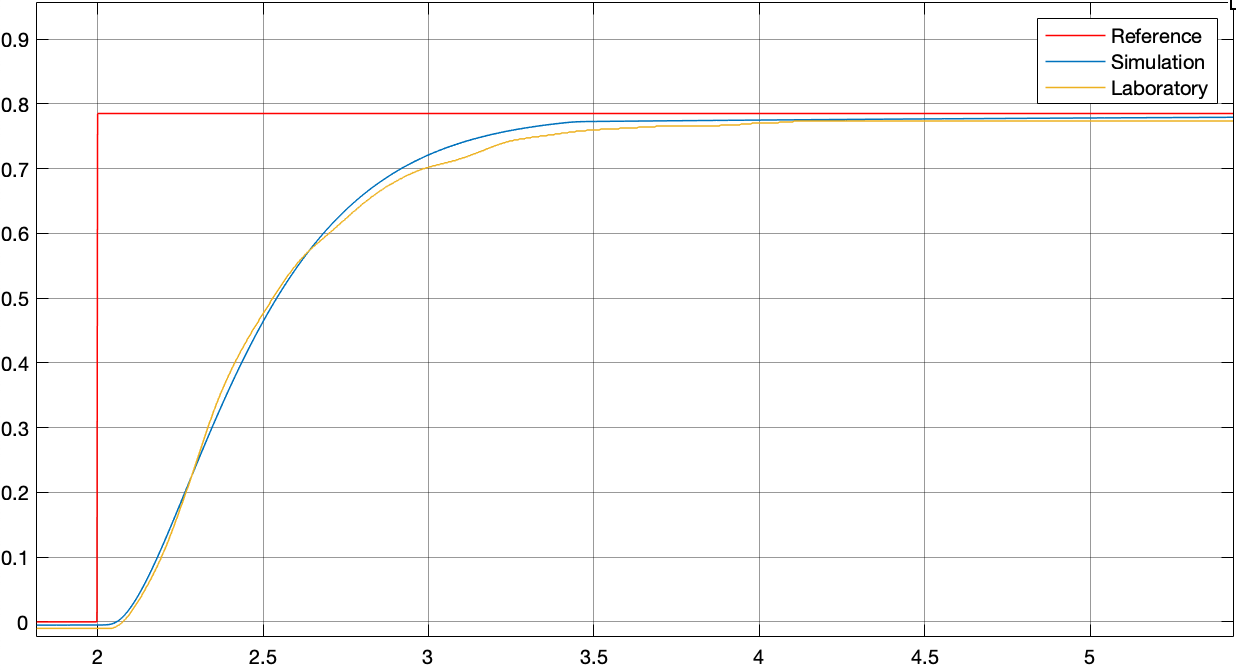
\includegraphics[width=\textwidth]{step_P_2dof}
		\subcaption{Position}
	\end{subfigure}
	\begin{subfigure}{0.45\columnwidth}
		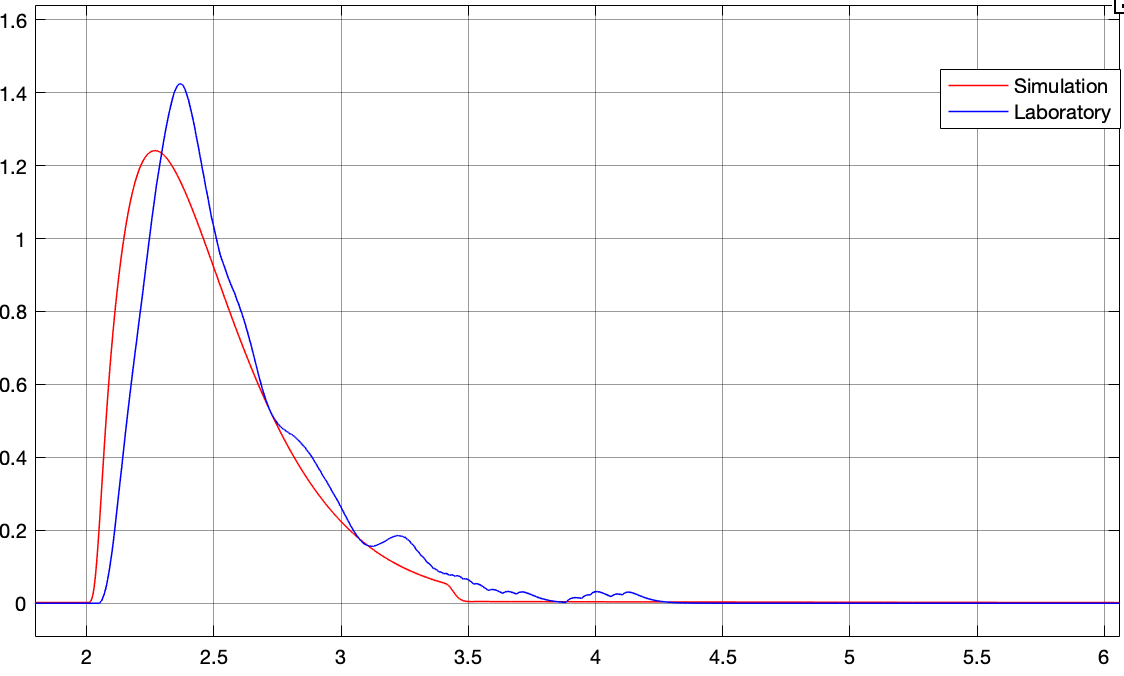
\includegraphics[width=\textwidth]{speed_P_2dof}
		\subcaption{Speed}
	\end{subfigure}
	\begin{subfigure}{0.45\columnwidth}
		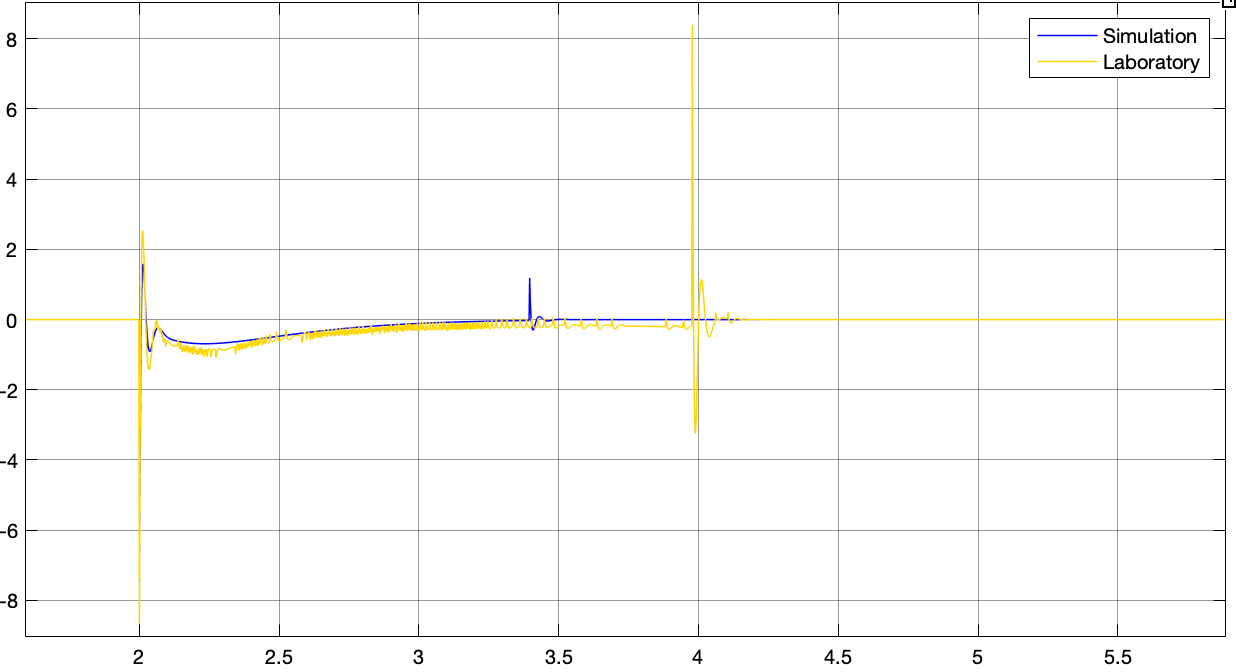
\includegraphics[width=\textwidth]{volt_P_2dof}
		\subcaption{Voltage}
	\end{subfigure}
	\caption{Position control loop with $k_{p} =2$ with a position step of $\frac{\pi}{4}$}
	\label{fig:P_2dof}
\end{figure*}
\newline
From \cref{fig:P_2dof}(c), it can observed the presence of two voltage spikes, which do not influence neither the position or the speed of the mass. As done in the \onedof\ position control, a logic switch is inserted in the PI controller to overcome the static friction issue, by disabling the integrator. This switch might be the cause of those spikes, indeed, these events arise whenever the switch is activated. 
It is possible to notice in \cref{fig:P_2dof}, that the second mass does not reach the position reference due to the above-mentioned switch gate.
The mismatch between the simulation and the laboratory data is fully negligible, as it is shown through the sinesweep experiment in \cref{fig:sinesweep_pos_2dof}. In also, from this sinesweep experiment the bandwidth of the closed loop system has been estimated to be equal to $w_{c,p}=2.7$, both for the simulation and the laboratory data.
\begin{figure*}[h]
	\centering
	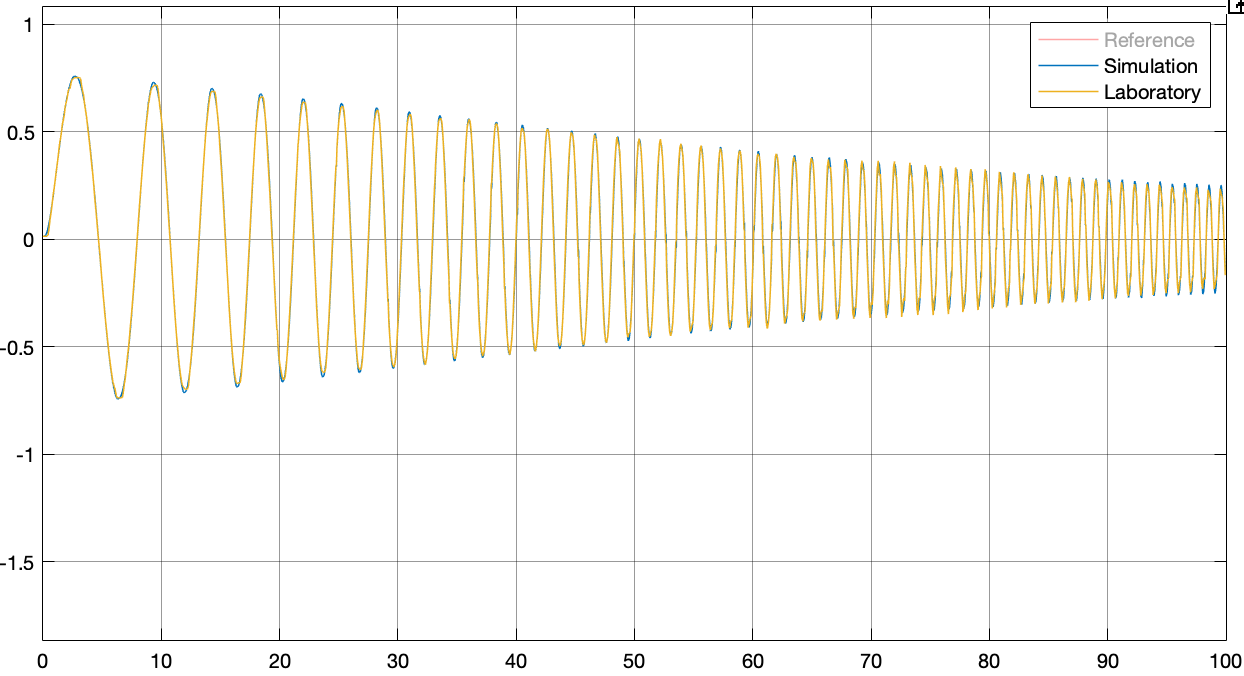
\includegraphics[scale=0.2]{sine_P_2dof}
	\caption{Sineweep experiment from $0.1\ Hz$ to $1\ Hz$ in $100\ s$}
	\label{fig:sinesweep_pos_2dof}
\end{figure*}